%%
\documentclass[preprint,12pt]{elsarticle}
\usepackage{hyperref}
%\hypersetup{
%	colorlinks=true,
%	linkcolor=blue,
%	filecolor=magenta,      
%	urlcolor=cyan,
%}
\usepackage{amsmath}
%% Use the option review to obtain double line spacing
%% \documentclass[preprint,review,12pt]{elsarticle}

%% Use the options 1p,twocolumn; 3p; 3p,twocolumn; 5p; or 5p,twocolumn
%% for a journal layout:
%% \documentclass[final,1p,times]{elsarticle}
%% \documentclass[final,1p,times,twocolumn]{elsarticle}
%% \documentclass[final,3p,times]{elsarticle}
%% \documentclass[final,3p,times,twocolumn]{elsarticle}
%% \documentclass[final,5p,times]{elsarticle}
%% \documentclass[final,5p,times,twocolumn]{elsarticle}
%\usepackage{feynmp}
\DeclareGraphicsRule{*}{mps}{*}{}
\usepackage[compat=1.1.0]{tikz-feynman}
\providecommand{\LuaTeX}{Lua\TeX}
\providecommand{\tikzfeynmanname}{\tikzname-Feynman}

%% if you use PostScript figures in your article
\usepackage{url}
%% use the graphics package for simple commands


\usepackage{graphics}
%% or use the graphicx package for more complicated commands
\usepackage{graphicx}
%% or use the epsfig package if you prefer to use the old commands
%% \usepackage{epsfig}
%%\usepackage{pifont}%use circled number
\usepackage{booktabs}
\usepackage{longtable}
\usepackage{multirow}
\usepackage{subfig}
%% The amssymb package provides various useful mathematical symbols
\usepackage{amssymb}
%% The amsthm package provides extended theorem environments
%% \usepackage{amsthm}

%% The lineno packages adds line numbers. Start line numbering with
%% \begin{linenumbers}, end it with \end{linenumbers}. Or switch it on
%% for the whole article with \linenumbers after \end{frontmatter}.
%% \usepackage{lineno}

%% natbib.sty is loaded by default. However, natbib options can be
%% provided with \biboptions{...} command. Following options are
%% valid:

%%   round  -  round parentheses are used (default)
%%   square -  square brackets are used   [option]
%%   curly  -  curly braces are used      {option}
%%   angle  -  angle brackets are used    <option>
%%   semicolon  -  multiple citations separated by semi-colon
%%   colon  - same as semicolon, an earlier confusion
%%   comma  -  separated by comma
%%   numbers-  selects numerical citations
%%   super  -  numerical citations as superscripts
%%   sort   -  sorts multiple citations according to order in ref. list
%%   sort&compress   -  like sort, but also compresses numerical citations
%%   compress - compresses without sorting
%%
%% \biboptions{comma,round}

% \biboptions{}

\numberwithin{equation}{section}
\begin{document}

\begin{frontmatter}

%% Title, authors and addresses

%% use the tnoteref command within \title for footnotes;
%% use the tnotetext command for the associated footnote;
%% use the fnref command within \author or \address for footnotes;
%% use the fntext command for the associated footnote;
%% use the corref command within \author for corresponding author footnotes;
%% use the cortext command for the associated footnote;
%% use the ead command for the email address,
%% and the form \ead[url] for the home page:
%%
%% \title{Title\tnoteref{label1}}
%% \tnotetext[label1]{}
%% \author{Name\corref{cor1}\fnref{label2}}
%% \ead{email address}
%% \ead[url]{home page}
%% \fntext[label2]{}
%% \cortext[cor1]{}
%% \address{Address\fnref{label3}}
%% \fntext[label3]{}

\title{Neutrino Studies and the SNO+ Experiment\\
	Doctoral Candidacy Exam Report
	}

%% use optional labels to link authors explicitly to addresses:
%% \author[label1,label2]{<author name>}
%% \address[label1]{<address>}
%% \address[label2]{<address>}

\author{Jie\quad Hu}

\address{Department of Physics, University of Alberta}

\end{frontmatter}

%%
%% Start line numbering here if you want
%%
% \linenumbers

%% main text
\section{Introduction}

\subsection{Research Backgrounds}
Neutrinos are one type of elementary particle in the Standard Model. The Standard Model is a theory describing elementary particles and their interactions. It has triumphantly passed various experimental verifications, including the discovery of Higgs bosons in 2012 and has ruled over the field of particle physics for more than 40 years. However, it has been found in experiments that some properties of neutrinos can not be described by the Standard Model, which shows clues of the new physics beyond the Standard Model. This put the studies of neutrinos in the spotlight.

SNO+ is one of the experiments for exploring the unknown properties of neutrinos. Its main research target is to examine the nature of neutrinos: whether they are Majorana or Dirac particles.

\subsection{Early Experiments}
The existence of neutrinos was first put forward by Wolfgang Pauli in 1930s to solve the contradictions observed in beta decay experiments. It was shown definitively by James Chadwick in 1914 that the electrons emitted in beta decay did not have a discrete set of energies but a continuous spectrum\cite{cowanexpintro}. This means that the energy, momentum and angular momentum (spin) were not conserved between the nucleus and electron. Pauli introduced a charge-neutral, spin 1/2 and nearly massless new particle. The sum of the energies of the new particle, the nucleus and electron is constant, which solved the problem. 

In 1934, Bethe and Peierls suggested direct neutrino detection via a neutrino-induced interaction, the inverse beta decay (IBD): $\bar{\nu}_e+p\to e^+ + n$. Their calculation showed the IBD cross section of the order of $10^{-43}~cm^2$. It indicates that the neutrino is difficult to be detected\cite{bethe1}.
 
However, in 1956, by utilizing a nuclear reactor as an intense neutrino source with neutrino fluxes on the order of $10^{12}-10^{13}$ neutrinos/second/cm$^2$, Fred Reines and Clyde Cowan made a first discovery of the neutrino (specifically, it was electron antineutrinos $\bar{\nu}_e$). Antineutrinos from a reactor interacted with the detector tank via IBD. As the tank was filled with water dissolved with cadmium chloride (CdCl$_2$), the produced positrons quickly annihilate with $e^-$ via pair-annihilation and gives $\gamma$ signals while the produced neutrons go through the neutron capture process: \noindent$n+^{108}$Cd$\to ^{109}$Cd$^*\to ^{109}$Cd$ +\gamma$ and gives delayed $\gamma$ signals. In addition, the water tank was surrounded by liquid scintillators coupled with photomultiplier tube (PMT) to detect emitted photons. A coincidence of these two characteristic signals, provides a distinctive signature for the neutrino reaction. They measured the cross-section as $6.3\times10^{-44}~cm^2$.

In the 1930s, Bethe et al. explained the origin of the Sun's energy is a series of nuclear reactions\cite{bethe2}. In 1964, John Bahcall pointed out that the direct evidence for the existence of nuclear reactions in the interiors of stars can only be proved by the detection of solar neutrinos. The endothermic reaction $\nu_e+^{37}$Cl$\to^{37}$Ar$+e^-$ was the most promising method for solar neutrinos detection. He also predicted the number of absorptions of solar neutrinos by terrestrial $^{37}$Cl atoms\cite{bahcall1}. In the meantime, Raymond Davis designed an experiment that used a 380 m$^3$ tank filled with Perchloroethylene (C$_2$Cl$_4$), a dry-cleaning fluid rich in chlorine. Solar neutrinos are expected to change $^{37}$C1 to $^{37}$Ar and the produced $^{37}$Ar were extracted and counted. The neutrino energy threshold ($E_{thresh}$) of the experiment is 0.814 MeV, which allows a measurement mostly of $^8$B neutrino fluxes but also including some lower energy neutrinos\cite{raymond}. Their first results announced in 1968 showed that only about one third of of the predicted radioactive argon atoms were measured, this raised a problem of missing solar neutrinos. 

Later in 1990s, GALLEX and SAGE measured lower energy solar neutrinos via the gallium reaction: $\nu_e+^{71}$Ga$\to^{71}$Ge$+e^-$, with an $E_{thresh}$ = 233.2 keV. This low threshold enables the gallium experiments to detect pp neutrinos, which constitute about 90\% of the neutrinos predicted by standard solar models. The results of the gallium experiments further confirmed the discrepancies as well as provided fundamental constraints on solar models\cite{GALLEX,SAGE,bahcall2}.

Cosmic rays from outer space continuously interact with nuclei in the atmosphere and produce secondary particles. Atmospheric neutrinos come from decay products of the hadrons in the secondaries. The dominate processes of atmospheric $\nu_e$ and $\nu_\mu$ production is $\pi^+\to\mu^+ + \nu_\mu$ followed by $\mu^+ \to e^+ + \bar{\nu}_\mu + \nu_e$. In the 1980s, Kamiokande in Japan was one of the experiments that was able to measure atmospheric neutrinos. They used a 3- kilo-tonne water-Cherenkov detector to count the Cherenkov rings caused by neutrino charged current interactions in the detector. The $\nu_e$ interaction produces an electron that produces an electro-magnetic shower during its propagation in the water while the $\nu_\mu$ interaction produces a muon that propagates almost in a straight line without producing electro-magnetic shower. Then $\nu_\mu$ ($\mu$-like events) are separated from $\nu_e$ ($e$-like events) by the fact that $\mu$-like events create sharper Cherenkov rings. Kamiokande measured the ratio of fluxes $\Phi(\nu_\mu+\bar{\nu}_\mu)/\Phi(\nu_e+\bar{\nu}_e)$. The fluxes of atmospheric neutrinos are well understood and the ratio $\nu_\mu/\nu_e$ is expected to be $\sim$2 at low energies $\leq$1~GeV. In 1988, they found a deficit of measured $\mu$-like events compared to the prediction, which was later confirmed by IMB in 1992\cite{imb} and Soudan-2 in 1997\cite{soudan2} and called ``atmospheric neutrino anomaly''\cite{atmNuReview}. In the meantime, by the ability to detect directional information of particles, they were able to observe the solar neutrinos by checking whether neutrinos were pointing away from sun. They also found that only about 1/2 of $^8$B solar neutrino flux was measured compared to the solar models\cite{kamioII}. 

\section{Neutrino Flavor Mixing and Conversion}
\subsection{SNO and Super-Kamiokande}
The facts of missing solar neutrinos and missing atmospheric neutrinos indicate that a neutrino can change its flavor or oscillate during propagation.

To resolve the solar neutrino problem with a direct approach, Herbert Chen in 1984 proposed an experiment using a large heavy water (D$_2$O) Cherenkov detector to distinguish the flavors of solar neutrinos\cite{herbertChen}. This proposal lead to the SNO collaboration. The SNO detector was sensitive to solar neutrinos from $^8$B decay via three interactions: (1) the charged current (CC): $\nu_e+d\to e^-+p+p$ , (2) the neutral current (NC): $\nu_x+d\to\nu+p+n$, (3) the elastic scattering (ES): $\nu_x+e^-\to \nu_x+e^-$. The CC channel is only sensitive to $\nu_e$ while the NC is independent of the neutrino type, which can provide a measurement of the total solar neutrino flux even if neutrinos change flavor. The ES channel is also sensitive to all flavors but with reduced sensitivities to $\nu_\mu$ and $\nu_\tau$\cite{SNO}.

In 2002, SNO reported that the measured total $^8$B solar neutrino flux ($\Phi_{NC}$) is consistent with solar models while the $\nu_e$ component of the flux ($\Phi_e$) is about 1/3 of the $\Phi_{NC}$\cite{SNO}:
\[
P_{SNO} = \frac{\Phi_e}{\Phi_{NC}}= 0.340\pm0.023^{+0.029}_{-0.031}
\]

These results indicate that about 2/3 of the original solar $\nu_e$ have transformed to $\nu_{\mu,\tau}$ when they arrived the earth. This explains the problem of missing solar neutrinos. The final results of SNO published in 2013\cite{SNOresult} for $^8$B neutrino flux are:
\[
\Phi_{total} = \sum_{f=e,\mu,\tau}\Phi(\nu_f)= 5.25\pm0.16(stat.)_{-0.13}^{+0.11}(sys.)\times10^6~cm^{-2}s^{-1}
\]
\[\Phi(\nu_\mu)+\Phi(\nu_\tau)=(3.26\pm0.25^{+0.40}_{-0.35})\times 10^6~cm^{-2}s^{-1}
\]

In 1996, the Kamiokande experiment was upgraded to a 50-kilo-tonne water Cherenkov detector, Super-Kamiokande (Super-K). In two years, Super-K measured sufficient atmospheric neutrinos and announced a striking discovery: the number of high energy muon neutrinos is zenith angle dependent and caused a deficit of up-going $\nu_\mu$. 

The measured up-going muon neutrinos are mostly created in the atmosphere at the opposite side of the Earth to the Super-K detector and travel about 12800 km while the downward-going muon neutrinos are created in the atmosphere about 15 km above the detector. The measured $\nu_e$ in the same scenario do not show such a deficit.

Therefore, a natural explanation for the results is that the up-going muon neutrinos have oscillated to $\nu_\tau$ during their thousands of kilometres travel. The Super-K results are consistent with two-flavor $\nu_\mu\leftrightarrow\nu_\tau$ oscillations\cite{superK}.


\subsection{Flavor Mixing Matrix and Oscillation Probability}
Both SNO and Super-K discovered the phenomenon of neutrino flavor conversions directly and were awarded the 2015 Nobel Prize. The phenomenon proves that neutrino has a small but finite mass. The violation of lepton number conservation is not expected in the Standard Model. Actually, as early as 1957, Pontecorvo had already suggested an oscillation of $\nu\leftrightarrow\bar{\nu}$, and later worked out a phenomenological model for $\nu_e\leftrightarrow\nu_\mu$ in theory\cite{nobeldoc}. In 1962, Ziro Maki, Masami Nakagawa and Shoichi Sakata further introduced a lepton mixing matrix (usually called PMNS matrix), which is a unitary transformation relating the neutrino flavor and mass eigenstates, to detail the neutrino oscillation phenomenon.

The flavor of a neutrino is determined as a superposition of the mass eigenstates. The two-flavor neutrino mixing model in vacuum is a simplified way to discuss the phenomenon of neutrino flavor conversion.

For a mixing of $\nu_e$ and $\nu_\mu$, we have a $2\times2$ unitary matrix of a parameter $\theta$ to relate the flavor eigenstates to the mass eigenstates\cite{cahn}:
\begin{equation}\label{eq:2flavormatrix}
\begin{bmatrix}
\nu_e\\
\nu_\mu\\
\end{bmatrix}
= U\begin{bmatrix}
\nu_1\\
\nu_2\\
\end{bmatrix}, ~~U=\begin{bmatrix}
\cos\theta &\sin\theta\\
-\sin\theta &\cos\theta\\
\end{bmatrix}
\end{equation}

Consider the time evolution: $\nu_i(t) = e^{-iE_it}\nu_i(0)~(i = 1,2)$ (use natural unit, $\hbar=c=1$), we have:
\begin{equation}
\begin{aligned}
|\nu_e(t)> = \cos\theta e^{-iE_1t}|\nu_1>+\sin\theta e^{-iE_2t}|\nu_2>
\\
|\nu_\mu(t)> = -\sin\theta e^{-iE_1t}|\nu_1>+\cos\theta e^{-iE_2t}|\nu_2>
\end{aligned}
\end{equation}

Then the probability that a $\nu_e$ at time $t_0=0$ transforms to a $\nu_\mu$ at time t is:
\begin{equation}
P_{\nu_e\to\nu_\mu} = |<\nu_\mu(t)|\nu_e(0)>|^2= 2\sin^2\theta\cos^2\theta[1-\cos(E_2-E_1)t]
\end{equation}

For ultra-relativistic neutrinos, the momentum $|\vec{p}|=p\simeq E\gg m$, then $E_1\simeq p+\frac{m^2_1}{2p}$ and $E_2\simeq p+\frac{m^2_2}{2p}$, we have $E_2-E_1\simeq\frac{m_2^2-m_1^2}{2p}$,
then $P_{\nu_e\to\nu_\mu}$ can be simplified to be:
\begin{equation}\label{eq:oscillation}
P_{\nu_e\to\nu_\mu} = \sin^2( 2\theta)\sin^2(\frac{m_2^2-m_1^2}{4E}t)=\sin^2( 2\theta)\sin^2(\frac{\Delta m^2}{4E}L)
\end{equation}

We usually define a  squared-mass difference $\Delta m^2=m_2^2-m_1^2$. $L = t$ is the distance neutrino travels. 

The maximum oscillation effect requires that $\frac{\Delta m^2}{4E}L\sim \pi$, which gives an effective length $L^{osc}=4\pi E/\Delta m^2$.

If we restore the $\hbar$ and $c$ and convert the natural unit to international system of units(S.I), we have:
\[
\sin^2(\frac{\Delta m^2}{4E}t)~\mathrm{[natural~unit]} = \sin^2\frac{\Delta m^2c^4}{4E\hbar}\frac{L}{c}~\mathrm{[S.I]}
\]

Consider the commonly used units by experiments,
\[
\frac{(\Delta m\cdot c^2)^2}{eV^2}\cdot \frac{L}{km}\cdot\frac{GeV}{E}\cdot\frac{1}{4\hbar c}
\]

Finally we conclude that under the two-flavor mixing model, a neutrino with energy $E_\nu$, after flying for a distance of $L$, has an oscillation probability of: 
\begin{equation}
P_{\nu_e\to\nu_{\mu}}=\sin^2(2\theta)\sin^2\Big(\frac{1.27\Delta m^2[eV^2]L[km]}{E_\nu[GeV]}\Big)
\end{equation}
The survival probability is defined as:
\begin{equation}
P_{\nu_e\to\nu_e}=1-P_{\nu_e\to\nu_{\mu}}
\end{equation}

\subsection{Matter Effects}
Integrated over the energy spectrum, the averaged survival probability of two-flavor mixing model in vacuum for solar neutrino is $<P_{\nu_e\to\nu_e}> = 1- 0.5\sin^2\theta\geq 0.5$, however the SNO results give $P_{SNO}\simeq0.3$. Therefore, the vacuum oscillation is not sufficient to explain the solar neutrino problem. We have to consider matter effects, also called the Mikheyev-Smirnov-Wolfenstein (MSW) mechanism\cite{smirnov,smirnov_msw}. 

The matter effect is caused by neutrinos interacting with ambient electrons and nucleons in matter such as the Sun or the Earth. $\nu_e$ interacts with electrons via both charged weak current (exchanging $W$ boson) and neutral weak current ($Z$ boson) while $\nu_\mu$ and $\nu_\tau$ interact only by the neutral current. $\nu_e$ energy has an addition potential, $V_{CC} =\sqrt2G_Fn_e$, where $n_e$ is the number density of the electrons in matter and $G_F$ is the Fermi coupling constant for the weak interaction\cite{smirnov,smirnov_msw}.

In vacuum two-flavor mixing, the Schr\"{o}dinger equation in mass eigenstates is (in natural unit)\cite{xing}:
\begin{equation}\label{eq:2mass_simple}
i\frac{d}{dt}\begin{bmatrix}
\nu_1\\
\nu_2\\
\end{bmatrix}
=H_0
\begin{bmatrix}
\nu_1\\
\nu_2\\
\end{bmatrix},~~H_0 = \begin{bmatrix}
E_1 & 0\\
0 &E_2\\
\end{bmatrix}
\end{equation}

Consider the mixing equation (\ref{eq:2flavormatrix}), use  the approximation of $E_2-E_1\simeq\frac{\Delta m^2}{2E}$, then we can change equation (\ref{eq:2mass_simple}) to flavor basis by:
\begin{equation}\label{eq:2flavor_simple}
i\frac{d}{dt}\begin{bmatrix}
\nu_e\\
\nu_\mu\\
\end{bmatrix}
= UH_0U^+\begin{bmatrix}
\nu_e\\
\nu_\mu\\
\end{bmatrix}
=
H^f_0
\begin{bmatrix}
\nu_e\\
\nu_\mu\\
\end{bmatrix}
\end{equation}
where 
\begin{equation}\label{eq:H0f}
H^f_0 = \begin{bmatrix}
-\frac{\Delta m^2}{4E}\cos 2\theta & \frac{\Delta m^2}{4E}\sin 2\theta\\
\frac{\Delta m^2}{4E}\sin 2\theta &\frac{\Delta m^2}{4E}\cos 2\theta\\
\end{bmatrix}+\frac{(m_1^2+m_2^2)}{2}\begin{bmatrix}
1 & 0\\
0 &1\\
\end{bmatrix}
\end{equation}

To simplify the calculation, we can drop the second term of $H^f_0$ that is irrelevant to the neutrino flavor conversion. Add the matter effect into $H_0$, we have:
\begin{equation}\label{eq:Hm}
H_m = \begin{bmatrix}
-\frac{\Delta m^2}{4E}\cos 2\theta+\sqrt 2G_Fn_e & \frac{\Delta m^2}{4E}\sin 2\theta\\
\frac{\Delta m^2}{4E}\sin 2\theta &\frac{\Delta m^2}{4E}\cos 2\theta\\
\end{bmatrix}
\end{equation}

If we define a mixing angle in matter $\theta_m$ as:
\begin{equation}\label{eq:thetaM}
\tan 2\theta_m = \frac{\Delta m^2\sin2\theta}{\Delta m^2\cos2\theta-2\sqrt 2E G_Fn_e}
\end{equation}

Also, define an effective squared-mass difference in matter $\Delta m^2_m$ as:
\begin{equation}
\Delta m^2_m = \sqrt{(\Delta m^2\cos2\theta - 2\sqrt 2EG_Fn_e)^2+(\Delta m^2\sin2\theta)^2}
\end{equation}

By analogy with the mixing in vacuum, now we can write the mixing equation relating the energy eigenstates in matter ($\nu_{1m},\nu_{2m}$) to the flavor eigenstates with a diagonalized Hamiltonian:
\begin{equation}\label{eq:matter_mixing}
\begin{bmatrix}
\nu_e\\
\nu_\mu\\
\end{bmatrix}
= \begin{bmatrix}
\cos\theta_m & \sin\theta_m\\
-\sin\theta_m & \cos\theta_m \\
\end{bmatrix}
\begin{bmatrix}
\nu_{1m}\\
\nu_{2m}\\
\end{bmatrix}
\end{equation}

The probability of flavor conversion is:
\begin{equation}
P_{\nu_e\to\nu_{\mu}}=\sin^2(2\theta_m)\sin^2\Big(\frac{\Delta m_m^2L}{4E}\Big)
\end{equation}

The denominator in equation (\ref{eq:thetaM}) implies that there is a resonance condition:
\begin{equation}\label{eq:reson_condition}
V(n_e)=\frac{\Delta m^2\cos2\theta}{2E}
\end{equation}
For a given energy $E$, we have the resonance density:
\begin{equation}
n^{reson}_{e}=\frac{\Delta m^2\cos2\theta}{2\sqrt2G_FE}
\end{equation}
For a given density $n^0_e$, we can also get a resonance energy $E^{reson}(n^0_e)$ in the medium.
In this case, $\theta_m = \frac{\pi}{4}$ and two flavor neutrinos are maximally mixed. This is the resonance enhancement of oscillations\cite{smirnov,japan_text}.

For the $\nu_e$ produced in the center of the Sun, if density there is very high, $n_e\gg n^{reson}_e$, then $\theta_m\to\pi/2$ if the resonance condition (\ref{eq:reson_condition}) is satisfied (in the resonance channel). From (\ref{eq:matter_mixing}), $\nu_e\simeq\nu_{2m}$.
If the density is not constant but varies slowly enough (decreases adiabatically from the center to the surface), although $\nu_{1m},\nu_{2m}$ are not eigenstates, the transitions $\nu_{1m}\leftrightarrow \nu_{2m}$ are suppressed. In this situation, $\nu_{2m}$ does not change to $\nu_{1m}$ during the whole propagation. Meanwhile, $\theta_m=\theta_m(n(t),E)$ changes. From (\ref{eq:matter_mixing}), we can get $\nu_{2m} = \sin\theta_m\nu_e+\cos\theta_m\nu_\mu$. In the resonance channel, the components of two flavor $\nu$s are equal; when $n_e\ll n^{reson}_e$, the (\ref{eq:thetaM}) reduces to $\tan(2\theta)$, or $\theta_m\to\theta$, which indicates that the matter effect reduces to vacuum mixing, or $\nu_{2m}\to\nu_2$. Then the survival probability is simply: 
\begin{equation}\label{eq:adiabatic}
P_{\nu_e\to\nu_e}=|<\nu_e|\nu_2>|^2=\sin^2\theta
\end{equation}
This process is called adiabatic conversion\cite{smirnov}. 

\subsection{Three-flavor mixing}
For three-flavor neutrino mixing, we have:
\begin{equation}\label{eq:mixingmatrix}
|\nu_f> = \sum_{k=1}^3U^*_{fk}|\nu_k> 
\end{equation}
where $f=e,\mu,\tau$ and $k=1,2,3$. U is the PMNS matrix and can be parametrized as: 
$U_{PMNS} = $
\begin{equation}
\begin{bmatrix}
1 &0 &0\\
0 &\cos\theta_{23} &\sin\theta_{23}\\
0 &-\sin\theta_{23} &\cos\theta_{23}\\ 
\end{bmatrix}
\begin{bmatrix}
\cos\theta_{13} &0 &e^{-i\delta_{CP}}\sin\theta_{13}\\
0 &1 &0\\
e^{-i\delta_{CP}}\sin\theta_{13} &0 &\cos\theta_{13}\\ 
\end{bmatrix}
\begin{bmatrix}
\cos\theta_{12} &\sin\theta_{12} &0\\
-\sin\theta_{12} &\cos\theta_{12} &0\\
0 &0 &1\\ 
\end{bmatrix}
\end{equation}

From the three-flavor mixing in vacuum, we can derive a survival probability with some approximations:
\begin{equation}\label{eq:disappear}
P_{\nu_\mu\to\nu_\mu}\simeq 1-(\cos^4\theta_{13}\sin^2 2\theta_{23}+\sin^2 2\theta_{13}\sin^2\theta_{23})\sin^2\frac{\Delta m^2_{31}L}{4E}
\end{equation}
and the oscillation or appearance probability\cite{nakaya}:
\begin{equation}\label{eq:appear}
P_{\nu_\mu\to\nu_e}\simeq \sin^2 \theta_{23}\sin^2 2\theta_{13}\sin^2 \frac{\Delta m^2_{32}L}{4E}
\end{equation}

In PMNS matrix, we have four parameters: $\theta_{12}$ is mainly measured by solar and reactor experiments, while $\theta_{13}$ is measured by atmospheric and accelerator experiments. $\delta_{CP}$ is a CP violation term. In addition, there are two squared-mass differences, $\Delta m^2_{sol}\equiv\Delta m^2_{21}=m_2^2-m_1^2$ and $\Delta m^2_{atm}\equiv\Delta m^2_{32}=|m_3^2-m_2^2|$. Currently, these 6 parameters can only be determined by experiments. The sign of $\Delta m^2_{32}$ is also to be determined, which indicates a mass hierarchy problem of whether neutrino mass is normal hierarchy (NH, $\Delta m^2_{32}>0$) or inverted hierarchy (IH, $\Delta m^2_{32}<0$).

\subsection{Experimental Aspects for Mixing Parameters}

Before the SNO experiment, solar neutrino experiments such as GALLEX, had explored the parameter space of $\Delta m^2_{sol}$ and $\theta_{12}$. One of the solutions to explain the missing number of solar neutrinos is called ``large mixing angle (LMA)". It constrains $\sin^2 2\theta_{12}=0.6-0.9$, $\Delta m^2_{sol}=(0.4-3)\times 10^{-5} eV^2$. The SNO results favor this solution but can not rule out the other ones, such as ``small mixing angle" (SMA) and ``low mass, low probability" (LOW)\cite{japan_text}. This issue was solved by a reactor $\bar{\nu}_e$ experiment, Kamioka Liquid Scintillator Antineutrino Detector (KamLand).

Reactor $\bar{\nu}_e$ experiments use the $\bar{\nu}_e$ generated by $\beta$-decays of fission products from heavy isotopes (mainly $^{235}$U, $^{238}$U, $^{239}$Pu and $^{241}$Pu) in nuclear reactors. The $\bar{\nu}_e$ flux is almost pure and the energy of reactor $\bar{\nu}_e$ is several MeV. The detection channel is via IBD: $\bar{\nu}_e+p\to e^+ + n$, which has a threshold of 1.8 MeV. This kind of experiment mainly measures $\bar{\nu}_e$ disappearance\cite{pdg2018}.

In 2003, KamLand discovered the reactor $\bar{\nu}_e$ disappearance over a long baseline of 180 km at 99.95\% C.L. Utilizing liquid scintillator, the experiment detected coincident signals from the $e^+$ and the delayed 2.2 MeV $\gamma$ from neutron capture on a proton. For the detected $\bar{\nu}_e$ with $E_{\bar{\nu}_e}>3.4$ MeV, they found the ratio of observed events to the expected events without $\bar{\nu}_e$ disappearance to be $0.611\pm0.085(stat.)\pm0.041(syst.)$\cite{kamland}. If CPT invariance is assumed, their best-fit gives $\sin^2 2\theta_{12}=1.0$ and $\Delta m^2_{21}=6.9\times10^{-5} eV^2$. This result favored the LMA solution for the solar neutrino problem and ruled out all the other ones\cite{kamland}. 

Combined with solar neutrino data, more precise measurements obtained $\Delta m^2_{sol} = 7.59^{+0.21}_{-0.21}\times 10^{-5}eV^2$ and $\tan^2{\theta}_{sol}=0.47^{+0.06}_{-0.05}$\cite{kamland_measure}.
Using the ${\theta}_{sol}$, the MSW adiabatic conversion mechanism gives $P_{\nu_e\to\nu_e}\simeq 0.3$, which is consistent with the SNO results. Therefore, combined with KamLand and SNO measurements, the solar neutrino problem is solved by the LMA-MSW solution.

The mixing angle $\theta_{13}$ is also measured with reactor $\bar{\nu}_e$ experiments. They look for the disappearance over baselines of $O(1 km)$. In late 1990s, CHOOZ and Parlo Verde experiments set an upper limit of $\sin^2 2\theta_{13}<0.12$ at 90\% C.L.\cite{joseTextbook}.

In 2011, the Daya Bay Experiment was built and is able to measure $\theta_{13}$ with a sensitivity of $\sin^2 2\theta_{13}\sim 0.01$.
In 2012, Daya Bay reported the discovery of non-zero $\theta_{13}$ with a significance of 5.2$\sigma$, which was confirmed by RENO and Double Chooz experiments in the same year. A more recent value from Daya Bay is reported in 2016\cite{dayabayresults}, based on 1230 days of operation and $\bar{\nu}_e$ data from eight detectors, $\sin^2 2\theta_{13} = 0.0841\pm0.0027(stat.)\pm0.0019(syst.)$. This result is supported by the other two reactor experiments, Double CHOOZ and RENO. This high-precision result makes $\sin^2 2\theta_{13}$ the best measured mixing angle\cite{reactorNu}.

Atmospheric and accelerator neutrino experiments mainly measure neutrinos of GeV energy scale. Accelerator neutrino experiments usually use a high-energy proton accelerator to produce neutrino beams. The proton beam is guided to collide on a target (such as graphite and aluminium) and $\pi$ (dominantly) and $K$ mesons are created. $\nu_\mu$ or $\bar{\nu}_\mu$ are the dominant products from meson decay. The typical energy of accelerator $\nu_\mu$ or $\bar{\nu}_\mu$ is about several GeV\cite{stateofart}.

The Tokai to Kamioka (T2K) experiment in Japan uses $\nu$ beam from the JPARC accelerator. The 295 km away (lone baseline) SuperK detector is used as a far detector. It measures the $\nu_\mu$ ($\bar\nu_\mu$) disappearance $\nu_\mu\to\nu_\mu$ ($\bar{\nu}_\mu\to\bar{\nu}_\mu$) and appearance $\nu_\mu\to\nu_e$ ($\bar{\nu}_\mu\to\bar{\nu}_e$) simultaneously. In 2017, by analyzing three-flavor $\nu$ and $\bar{\nu}$, T2K rejects the hypothesis that neutrinos and antineutrinos oscillate with the same probability at 95\% confidence (2$\sigma$) level. This indicates a hint of CP symmetry broken by neutrinos. Their recent results give the region of $\delta_{CP}$ in [-2.95,-0.44] (NH) and [-1.47,-1.27] (IH) at 90\% C.L. Obviously, CP conserving values, $\delta_{CP} = 0,\pi$ are not in the measured region and are excluded. The measured NH (IH) parameters are: $\Delta m^2_{32}=2.54\pm 0.08~(-2.51\pm0.08)\times 10^{-3} eV^2$ and $\sin^2\theta_{23} = 0.55^{+0.05}_{-0.09}~(0.55^{+0.05}_{-0.08})$\cite{t2k}.

Both of the NOvA and the MINOS (currently is upgraded to MINOS+) experiments use NUMI accelerator neutrino beam at Fermi lab. Both experiments have measured $\Delta m^2_{32}$ and $\sin^2\theta_{23}$. In 2017, NOvA showed some tension with T2K results. Their data disfavored the maximal mixing of $\sin^2\theta_{23}$ at 2.6$\sigma$. This will be clarified in the future\cite{nova}.

As a typical atmosphere neutrino experiment, SuperK is sensitive to measure the parameters of $\Delta m^2_{32}$, $\sin^2\theta_{32}$ as well as $\delta_{CP}$. The most recent results from SuperK show that in NH, $\sin^2\theta_{23}=0.588^{+0.031}_{-0.064}$ and $\Delta m^2_{32} = 2.5^{+0.13}_{-0.20}\times 10^{-3} eV^2$\cite{superk_new}. 

Two kilometer-scale neutrino telescopes, IceCube and ANTARES, that are aimed to detect neutrinos originating from astronomical objects in the PeV range, have been measuring atmospheric neutrinos in the energy region above $O(10)$ GeV. Their results of $\Delta m^2_{32}$ and $\theta_{23}$ are consistent with those from atmosphere and accelerator experiments\cite{stateofart}.  

To conclude this section, future experiments are expected to make precise measurements to obtain the value of $\delta_{CP}$, the CP violation parameter of neutrino oscillations as well as to determine whether the mass hierarchy is normal or inverted.

\section{Double Beta Decay}

For heavy radioactive isotopes that are even-even nuclei, that is nuclei of even neutron number (N) and even proton number (Z), the beta decay will lead to an odd-odd nucleus which is less stable. For such isotopes the beta decay is energetically forbidden. In 1935, Maria Goeppert-Mayer pointed out that they can still decay through double beta decay process: $(Z,A) \to (Z+2,A)+2e^{-}+2\bar{\nu_e}$. This is called ordinary double beta decay or $2\nu\beta\beta$\cite{martin}.

In 1937, Ettore Majorana proposed that neutral spin-1/2 particles (fermions) can be their own antiparticles\cite{majorana}. In this case, the process called neutrinoless double beta decay ($0\nu\beta\beta$) is also expected. The Feynman diagrams of $2\nu\beta\beta$ and $0\nu\beta\beta$ are illustrated in Fig.~\ref{feynman1}.

\begin{figure}[htbp]
	\centering	
	\begin{minipage}[t]{0.45\textwidth}
	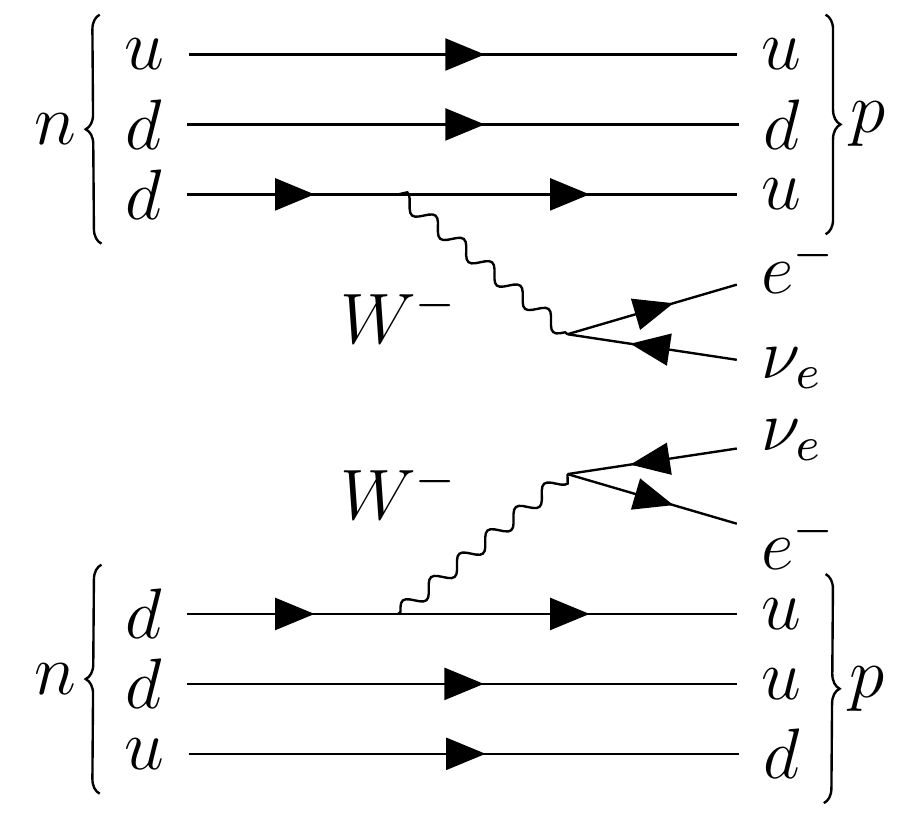
\includegraphics[width=5cm]{doubleBeta2nu_feynman.png}
	\end{minipage}
	\begin{minipage}[t]{0.45\textwidth}
	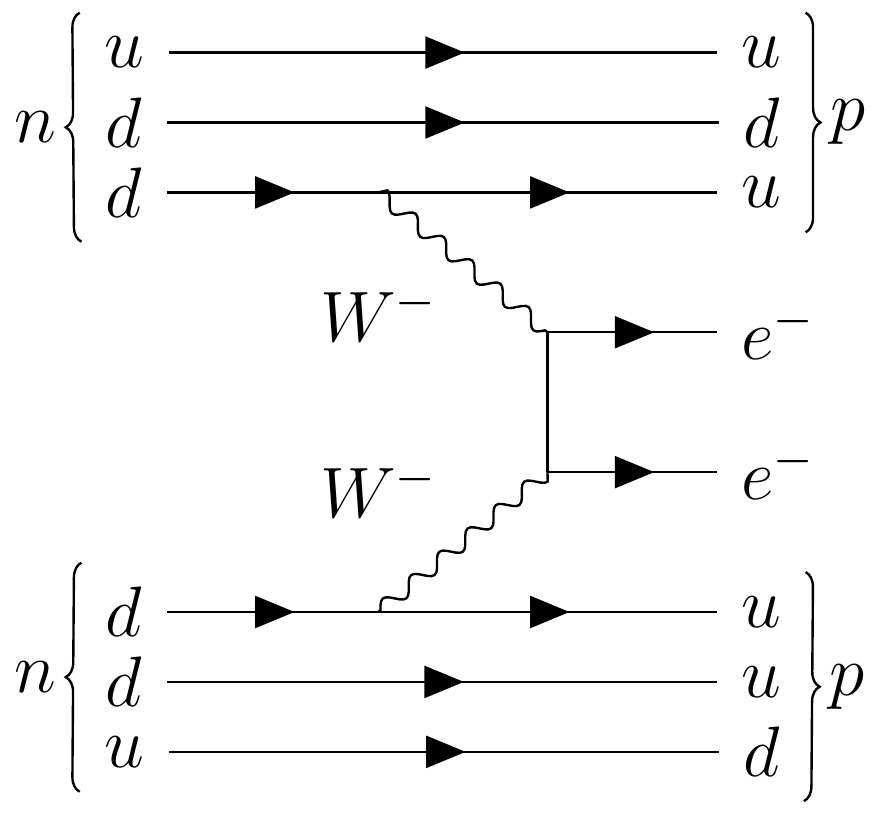
\includegraphics[width=5cm]{doubleBeta_feynman.png}
	\end{minipage}
	\caption{ Feynman diagrams for $2\nu\beta\beta$ (left) and $0\nu\beta\beta$ (right).}
	\label{feynman1}
\end{figure}

The interpretation of the $0\nu\beta\beta$ process is considered as exchanging light Majorana neutrinos. In this case the effective Majorana mass $<m_{ee}>=\sum_{i=1}^{3} |U_{ei}|^2m_i~(i=1,2,3)$, where $U_{ei}$ is the elements of the neutrino mixing matrix that defines the $\nu_e$ and $m_i$ is the mass eigenvalues of the mass eigenstates, from (\ref{eq:mixingmatrix}). The observable quantity for experiments is the half-life:
\[
(T^{0\nu\beta\beta}_{1/2})^{-1} = G_{PS}|M_{Nuclear}|^2<m_{ee}>^2 
\]
where $G_{PS}$ is the phase space, $|M_{Nuclear}|$ the nuclear matrix element for the physics process considered to describe the $0\nu\beta\beta$ decay process\cite{kaizuber}.

Similar to the beta decay, the $2\nu\beta\beta$ process will cause a continuous spectrum in the detector while the $0\nu\beta\beta$ process only has two electrons in the final state, which sum up to give a distinct energy peak. By measuring this exact energy, a detector with high energy resolution is able to search for the $0\nu\beta\beta$ signal from radioactive isotopes. Diverse technologies for the neutrino detection have been developed during the past decades.

\subsection{Status of Double Beta Decay Experiments}
The GERmanium Detector Array (GERDA) experiment searches for $0\nu\beta\beta$ of $^{76}$Ge. The experiment uses bare germanium crystals with an enrichment of up to $\sim$87\% $^{76}$Ge operated in a radiopure cryogenic liquid argon (LAr). GERDA Phase I had an exposure of 21.6 kg$\cdot$yr and Phase-II started with 35.6 kg from enriched material in December 2015. With combined data of Phase I and Phase II, GERDA reported in 2016 a lower limit half-life of $T^{0\nu}_{1/2}(^{76}$Ge$)>5.3\times 10^{25}$ years at 90\% C.L.\cite{gerda,gerda2}.

The Enriched Xenon Observatory (EXO) experiment uses 200-kg of liquid Xenon (LXe) in a time projection chamber (TPC) to search for $0\nu\beta\beta$ in $^{136}$Xe. In 2011 they observed the half life of $2\nu\beta\beta$ of $^{136}$Xe to be $2.11\times 10^{21}$ years. A limit of $T^{0\nu}_{1/2}(^{136}$Xe$)>1.1\times 10^{25}$ yr\cite{exo} was set in 2014. EXO is now being upgraded to the next 5-tonne experiment (nEXO) and is expected to reach an exclusion sensitivity of $T^{0\nu}_{1/2}(^{136}$Xe) of about $10^{28}$ years at 90\% C.L.\cite{nEXO}.

Also looking into $^{136}$Xe, the KamLAND-Zen experiment exploits the existing facilities of KamLAND by setting a 3.08-m-diameter spherical inner balloon filled with 13 tons of Xe-loaded liquid scintillator at the center of the KamLAND detector. Their 2016 results from a 504 kg$\cdot$yr exposure obtained a lower limit for the $0\nu\beta\beta$ decay half-life of $T^{0\nu}_{1/2}(^{136}$Xe$)>1.07\times 10^{26}$ yr at 90\% C.L. and the corresponding upper limits on the effective Majorana neutrino mass are in the range 61-165 meV\cite{kamlandZen}.

The Cryogenic Underground Observatory for Rare Events (CUORE) experiment searches for $0\nu\beta\beta$ in $^{130}$Te. CUORE is a tonne-scale cryogenic bolometer array that arranges 988 tellurium dioxide (TeO$_2$) crystals. CUORE reported first results in 2017 after a total TeO$_2$ exposure of 86.3 kg$\cdot$yr. Combined with their early data, they placed a lower limit of $T^{0\nu}_{1/2}(^{130}$Te$)>1.5\times 10^{25}$ yr at 90\% C.L. and $m_{\beta\beta}<(140-400)$  meV\cite{cuore}.

The sensitivities of $T^{0\nu}_{1/2}$ and $m_{\beta\beta}$ for current and future experiments are concluded in Fig.~\ref{biller}\cite{stevenbiller}.
\begin{figure}[htbp]
	\centering	
	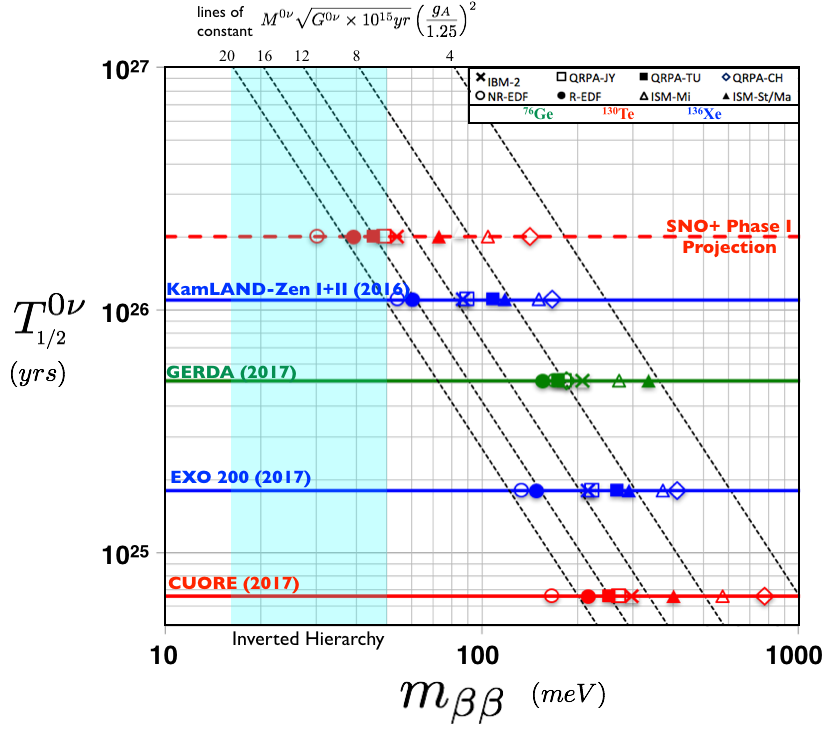
\includegraphics[width=8cm]{0nbbComparisonAug2017.png}
	\caption{Sensitivity of $T^{0\nu}_{1/2}$ for current and future experiments.}
	\label{biller}
\end{figure}

\section{SNO+ Experiment}
The SNO+ experiment is the successor of the SNO experiment, which makes use of the SNO detector structure. Located in SNOLAB at a depth of 2 km from the surface, the rock overburden is about 6000 meter water equivalent (m.w.e), which greatly reduces the cosmic muon backgrounds. The detector consists of an acrylic vessel (AV) sphere of 12 m in diameter and 5.5 cm in thickness. The AV sphere is concentric within a 17.8 m diameter stainless steel sphere, which holds 9438 photomultipliers (PMT). These two structures are housed in a rock cavity filled with 7000 tonnes of ultra-pure water (UPW) to provide both buoyancy for the vessel and radiation shielding\cite{whitepaper, erica}.

The SNO+ detector is designed for multi-purpose measurements of the neutrino physics.
The experiment will go through three phases\cite{whitepaper}: 

1. Water phase 

The AV was filled with about 900 tonnes of ultra-pure water. The detector has been collecting physics data since May 2017.

The main physics goal in this phase is to search for the invisible nucleon decay, which violates baryon number and is a prediction of Grand Unified Theory (GUT). In this decay mode, $^{16}$O decays into $^{15}$O$^*$ or $ ^{15}$O$^*$, which de-excites and produces a $\gamma$ ray of about 6 MeV.

During the water phase, different types of calibration runs have been operated. The detector responses, systematics and backgrounds are studied. Multiple physics analyses of solar neutrinos, reactor antineutrinos and nucleon decay are going on. The external backgrounds are also measured for the following two phases. 

2. Scintillator phase

The AV will be filled with 780 tonnes of liquid scintillator, which is a mixture of linear alkylbenzene (LAB) as solvent and 2 g/L of 2,5-diphenyloxazole (PPO) as fluor.

In this phase, the main physics goal is to measure low energy solar neutrinos: the CNO, pep, and low energy $^8$B neutrinos. Geo neutrinos, reactor antineutrinos and supernova neutrinos are also on the analysis list.

A six-month of scintillator filling and 6 months to a year data-taking is expected for this phase. During the filling, it is planned to operate the partially filled detector at a water level about 4.4 m for a short duration. This partial filled transition phase is mainly aimed to understand the background of scintillator. 

3. Tellurium loading phase

In this final phase, natural Tellurium will be loaded into the scintillator, in which $^{130}$Te is the double beta decay isotope. The main purpose in this phase is searching for $0\nu\beta\beta$ in $^{130}$Te.

\section{My Work on SNO+}
\subsection{Wavelength Shifter (WLS) Study}
There was a proposal of adding the wavelength shifter (WLS) into the SNO+ detector during the water phase. The specific wavelength shifter we considered is PPO, which will also be used in the SNO+ scintillator phase and Te-loaded phase. Although the proposal will not happen for SNO+ due to the experiment schedule, it is still worthwhile for a conceptual study of a SNO+-like detector that uses water-based wavelength shifter (wbWLS) as medium. The advantage of a wbWLS detector is to increase the light yield while still keeps the directionality. This technology is actually being studied by some future solar neutrino experiments, such as the Advanced Scintillation Detector Concept (ASDC)\cite{asdc}.

Fig.~\ref{pmt_wls} shows the PMT distributions of Monte Carlo (MC) simulated 5 MeV electrons travelling along one direction in the AV. The left plot shows the case when the detector is filled with pure water while the right plot is for water plus 0.1 ppm PPO. For the same electrons, the number of triggered PMTs (NHit) in waterPPO is about 2.4 times the case in pure water. Although there are extra isotropic lights emitted, the Cherenkov ring still can be seen clearly, which indicates the directionality can be reconstructed for analysis.  

\begin{figure}[htbp]
	\centering
	\begin{minipage}[t]{0.48\textwidth}
		\centering
		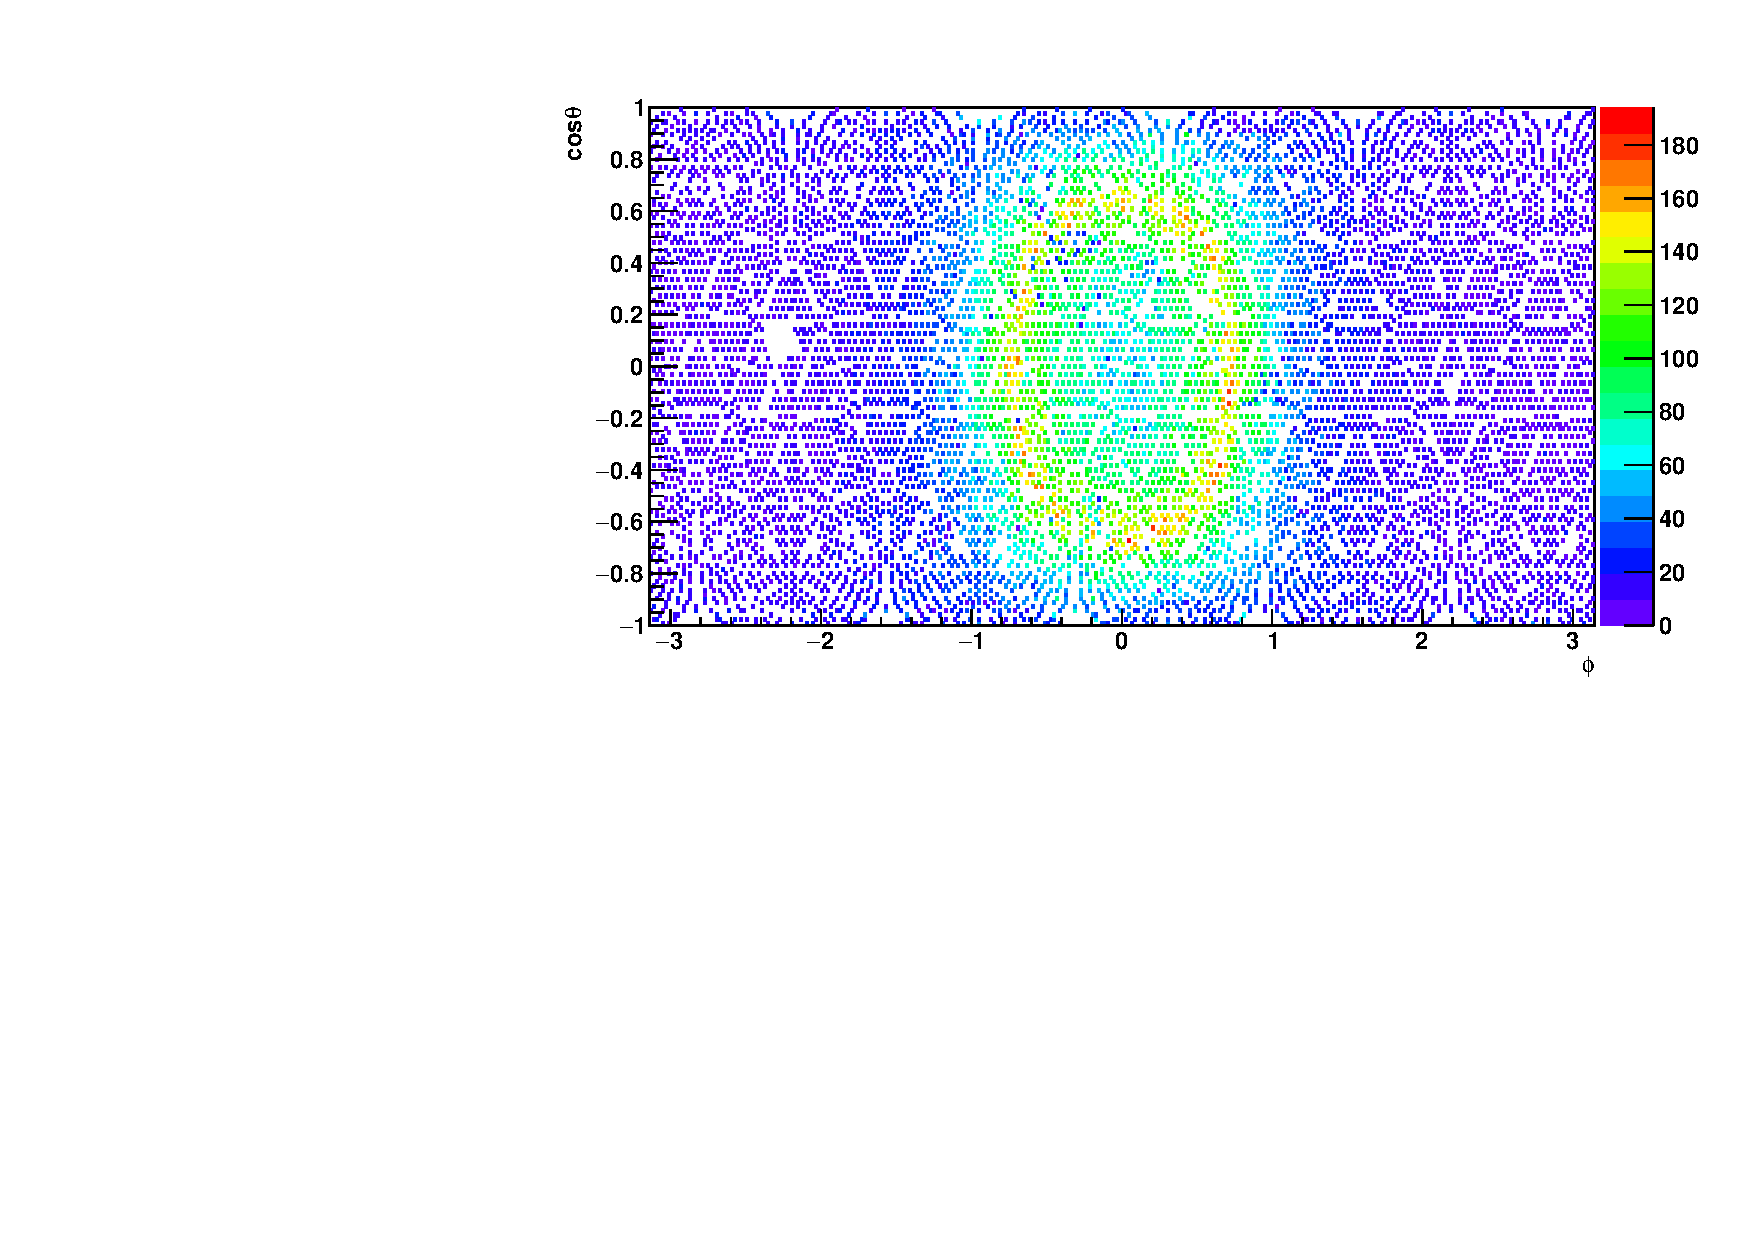
\includegraphics[width=7cm]{PMT_5MeVElectronWater.pdf}
	\end{minipage}
	\begin{minipage}[t]{0.48\textwidth}
		\centering
		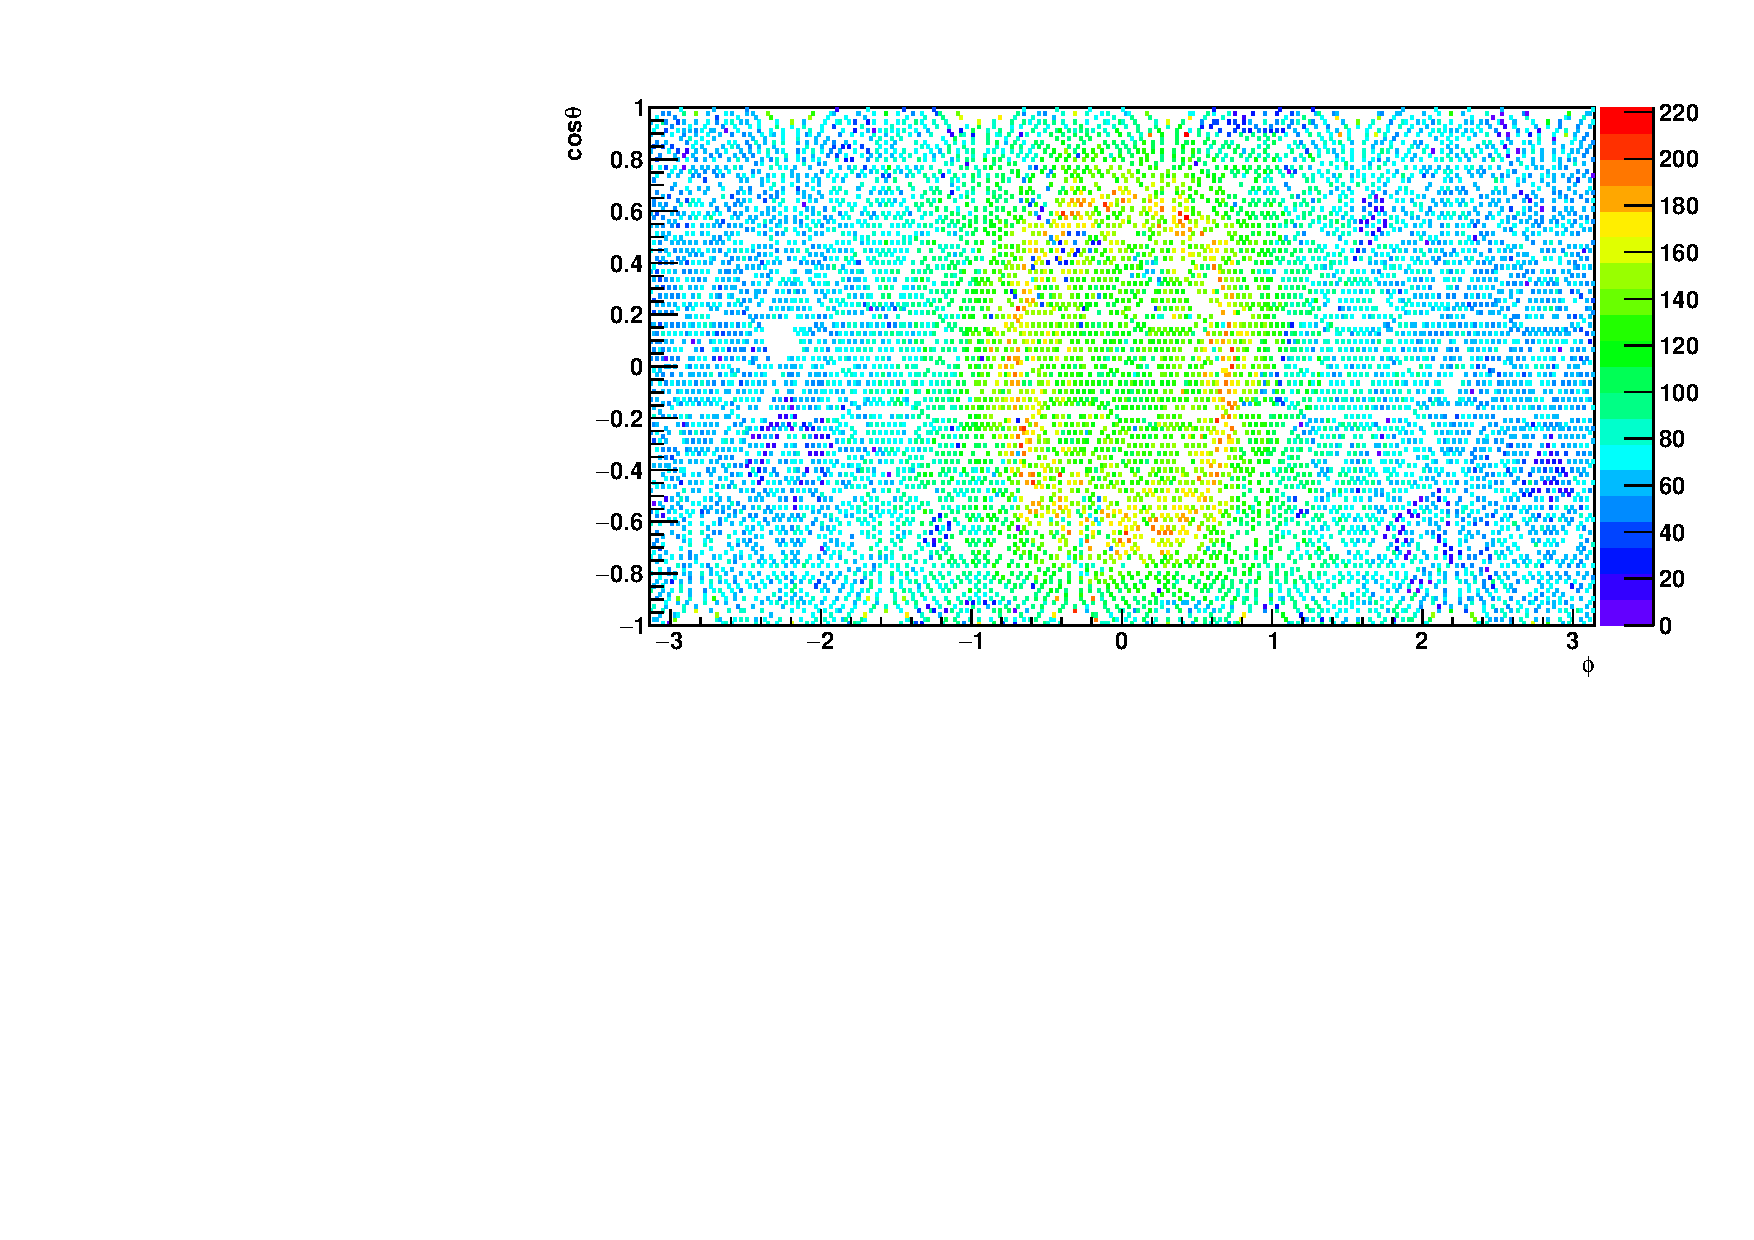
\includegraphics[width=7cm]{PMT_5MeVElectron0p1ppmPPO.pdf}
	\end{minipage}
	\caption{Distributions of PMT hit for 5 MeV electrons travelling along +x direction in the pure water (left); water plus 0.1 ppm PPO (right).}
	\label{pmt_wls}
\end{figure}

%The different amounts of water+bis-MSB and water+PPO samples were prepared at the University of Alberta and bench-top measurements were performed. Fig.~\ref{solution} shows different types of samples in front of UV light source. In pure water (leftmost panel), there is no fluorescent light; the bluish fluorescent lights from the water+WLS samples look similar.
%
%\begin{figure}[htbp]
%	\centering	
%	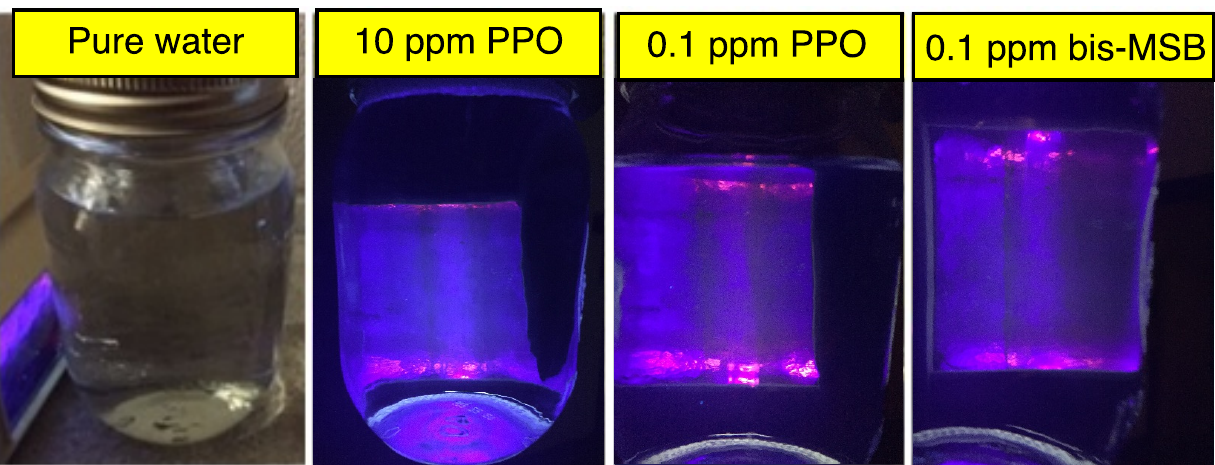
\includegraphics[width=10cm]{mergedPic.png}
%	\caption{ Pure water as well as WLS solutions placed in front of UV light source.}
%	\label{solution}
%\end{figure}

Fig.~\ref{nhit_wls} shows the energies of simulated electrons as a function of mean Nhits. We can see in pure water case, 1 MeV electron can not trigger any PMTs while in wbWLS case we have a mean Nhits of 20.

\begin{figure}[htbp]
	\centering	
	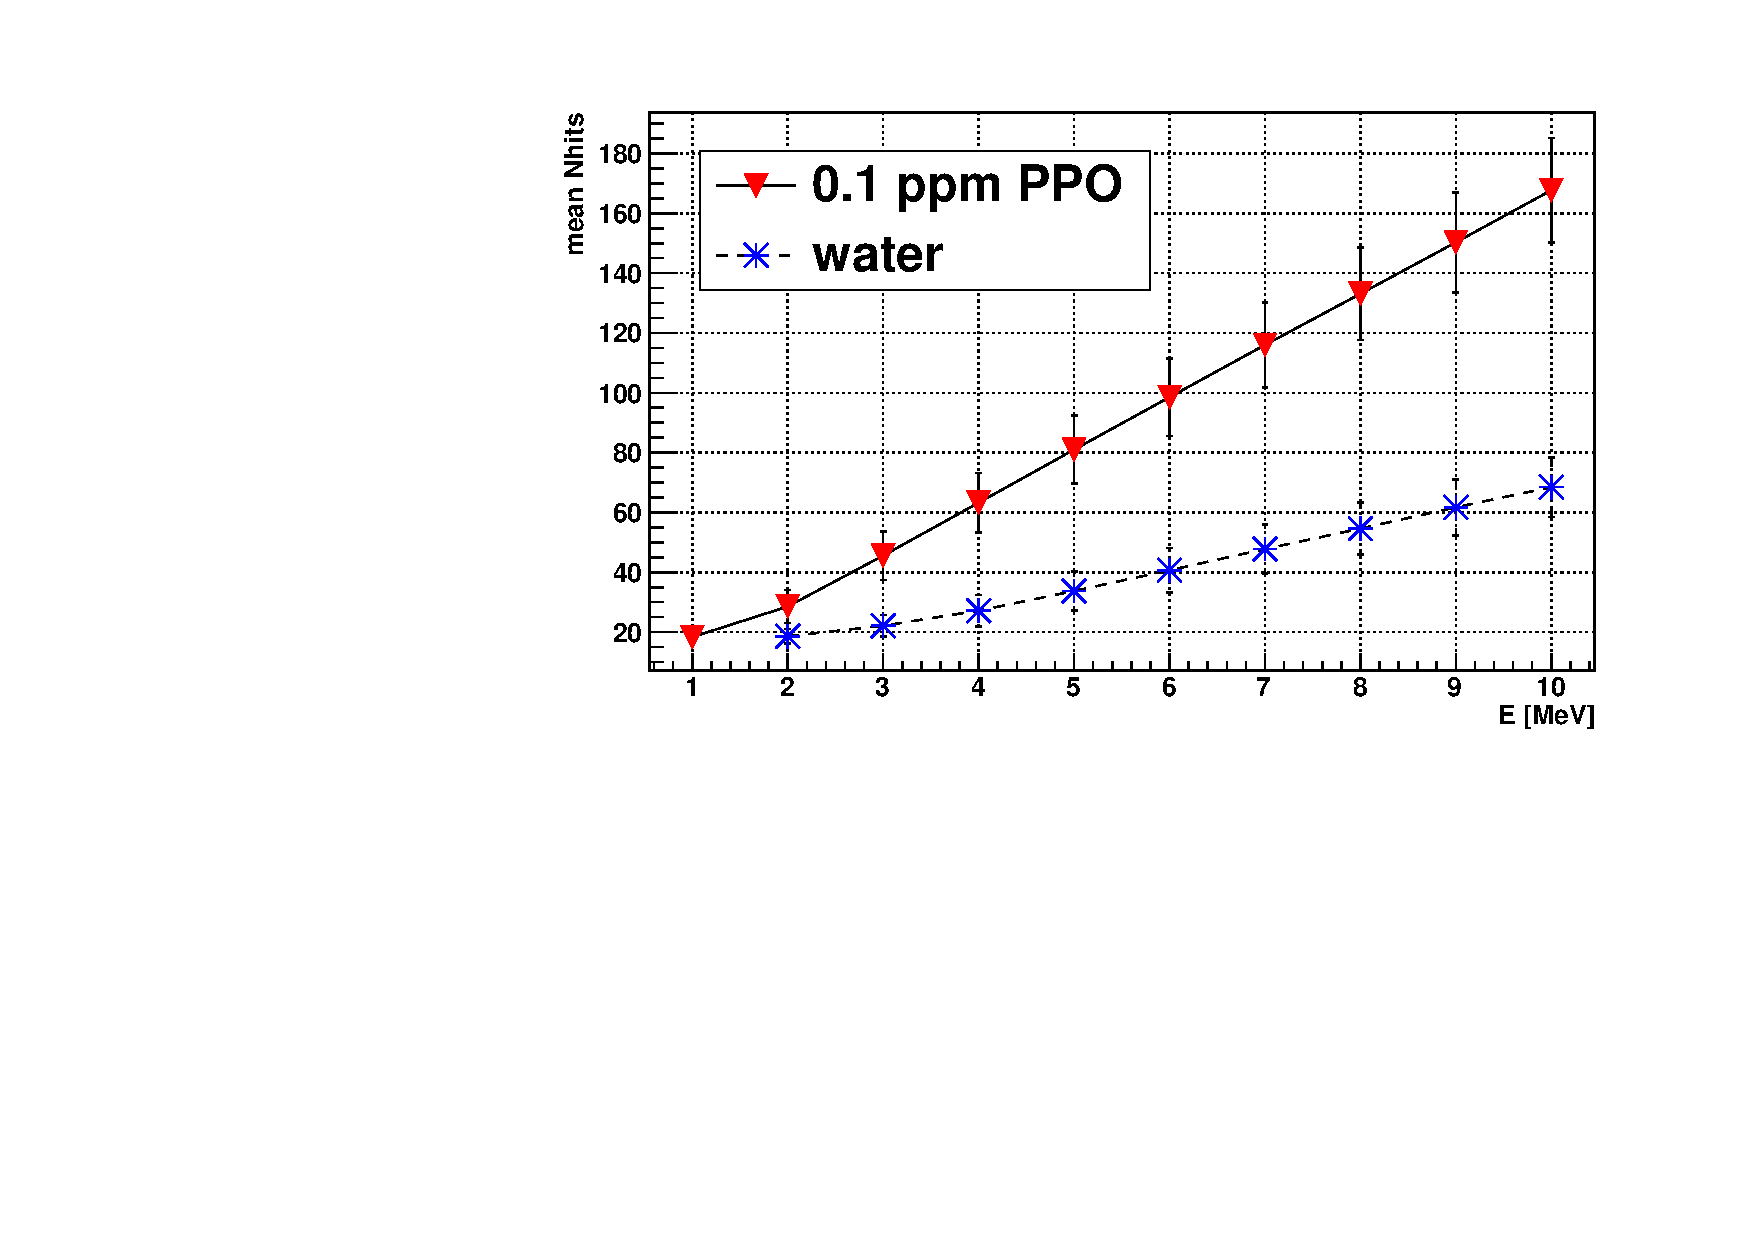
\includegraphics[width=8cm]{nhits_wls.pdf}
	\caption{ The energies of simulated electrons as a function of mean Nhits. The values in the 0.1 ppm PPO (solid line with inverted triangle) are compared with the water (dashed line with star).}
	\label{nhit_wls}
\end{figure}

To study the physics events in the wbWLS SNO+ detector, we need a reconstruction algorithm (fitter) to obtain the position, direction and time of an event. A Multi-path Fitter (MPF) framework was developed by the Alberta group as an alternative fitter for SNO+. The fitter uses prompt light and straight line paths for likelihood calculations. Fig.~\ref{mpwdiagram} shows the reconstruction concepts for position and direction. 

\begin{figure}[htbp]
	\centering
	\begin{minipage}[t]{0.4\textwidth}
		\centering
		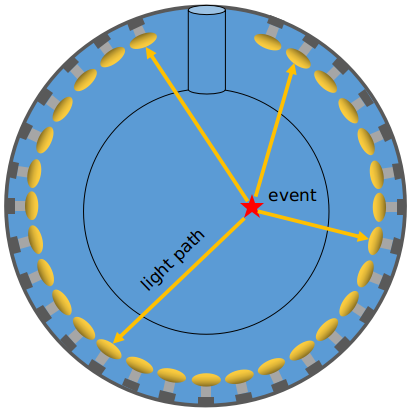
\includegraphics[width=4cm]{mpwDiagram.png}
	\end{minipage}
	\begin{minipage}[t]{0.4\textwidth}
		\centering
		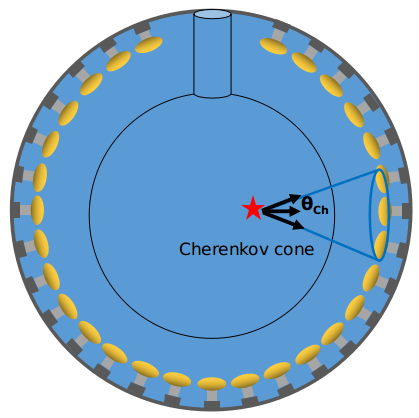
\includegraphics[width=4cm]{mpwDiagram2.png}
	\end{minipage}
	\caption{Diagrams of position reconstruction (left) and direction (right).}
	\label{mpwdiagram}
\end{figure}

In the left panel of Fig.~\ref{mpwdiagram}, when an event happens at a position of $\vec{X}_{0}$, photons are emitted and propagate to PMTs. The triggered PMTs at known positions $\vec{X}_\mathrm{PMT}$ record the arrival time of light ($t_\mathrm{PMT}$). A timing parameter, time residual, is defined by: 
\begin{equation}
t_{res} = t_\mathrm{PMT}-\frac{|\vec{X}_{0}-\vec{X}_\mathrm{PMT}|}{c_{average}}-t_0
\end{equation}
where $t_0$ is the event time and $c_{average}$ is an averaged group velocity ($v_{gr}$) of light.

For all the triggered PMTs, the likelihood is built by $L=\prod^{Nhit}_{i=0}P_i(t_{res})$. If we know the timing spectrum of PMT response to a certain detector optical property, we can use the timing spectrum as a probability density function (pdf). In the case here is the PMT timing response to the photon propagating in the wbWLS. This timing pdf is shown in the left panel of Fig.~\ref{WLS_pdf}.
The fitter varies the trial vertex $(\vec{X}_{0},t_0)$ to fit with the pdf. By maximizing the likelihood, the best-fit vertex is found.

A cone of Cherenkov photons is created along the charged particle momentum $\vec{p}$, or the direction of the particle, $\vec n = \vec p/|\vec p|$. The light cone is detected on the PMT sphere, forming a Cherenkov ring. For a known (or best-fit) $\vec{X}_{0}$ and triggered PMT position $\vec{X}_{PMT}$, the angle $\theta_{cone}$ between $(\vec{X}_{PMT}-\vec{X}_{0})$ and $\vec n$ is calculated by:
\[\cos\theta_\mathrm{cone} = \frac{(\vec{X}_\mathrm{PMT}-\vec{X}_{0})\cdot \vec{n}}{|\vec{X}_\mathrm{PMT}-\vec{X}_{0}|}\]
It should be close to the Cherenkov angle $\theta_{Ch}$. This is illustrated in the right panel of Fig.~\ref{mpwdiagram}. From the MC simulations of electrons travelling along the same direction in the pure water, we extract a distribution of $\cos\theta_{Ch}$ (angular distribution), as shown in the right panel of Fig.~\ref{WLS_pdf}. 

\begin{figure}[htbp]	
	\centering	
	\subfloat[Timing pdf for wbWLS position reconstruction.]{ 	
		\begin{minipage}[b]{0.5\textwidth}			
			%\centering			
			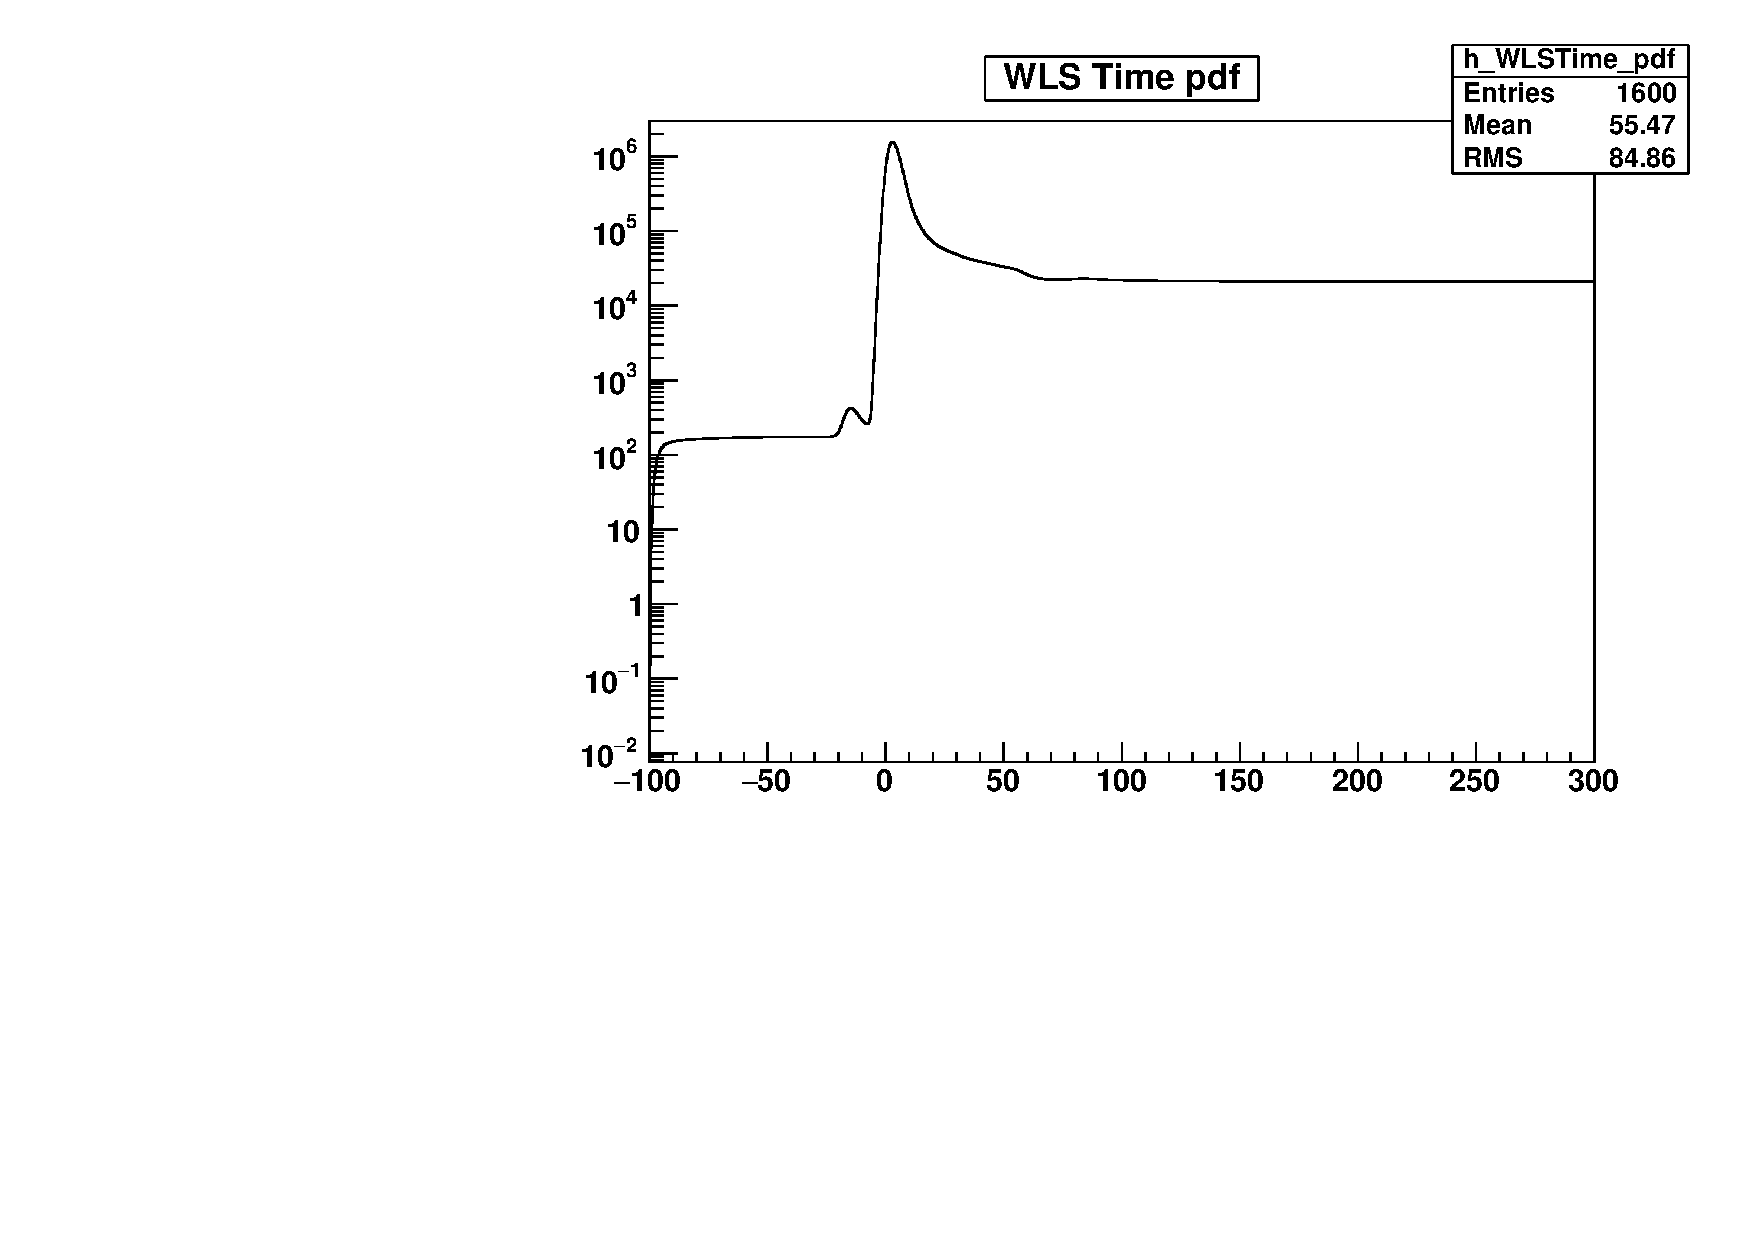
\includegraphics[width=7cm]{WLSTime_pdf.pdf}			
		\end{minipage}%		
	}% 	
	\subfloat[Agular pdf for direction reconstruction.]{		
		\begin{minipage}[b]{0.5\textwidth}		
			%\centering	
			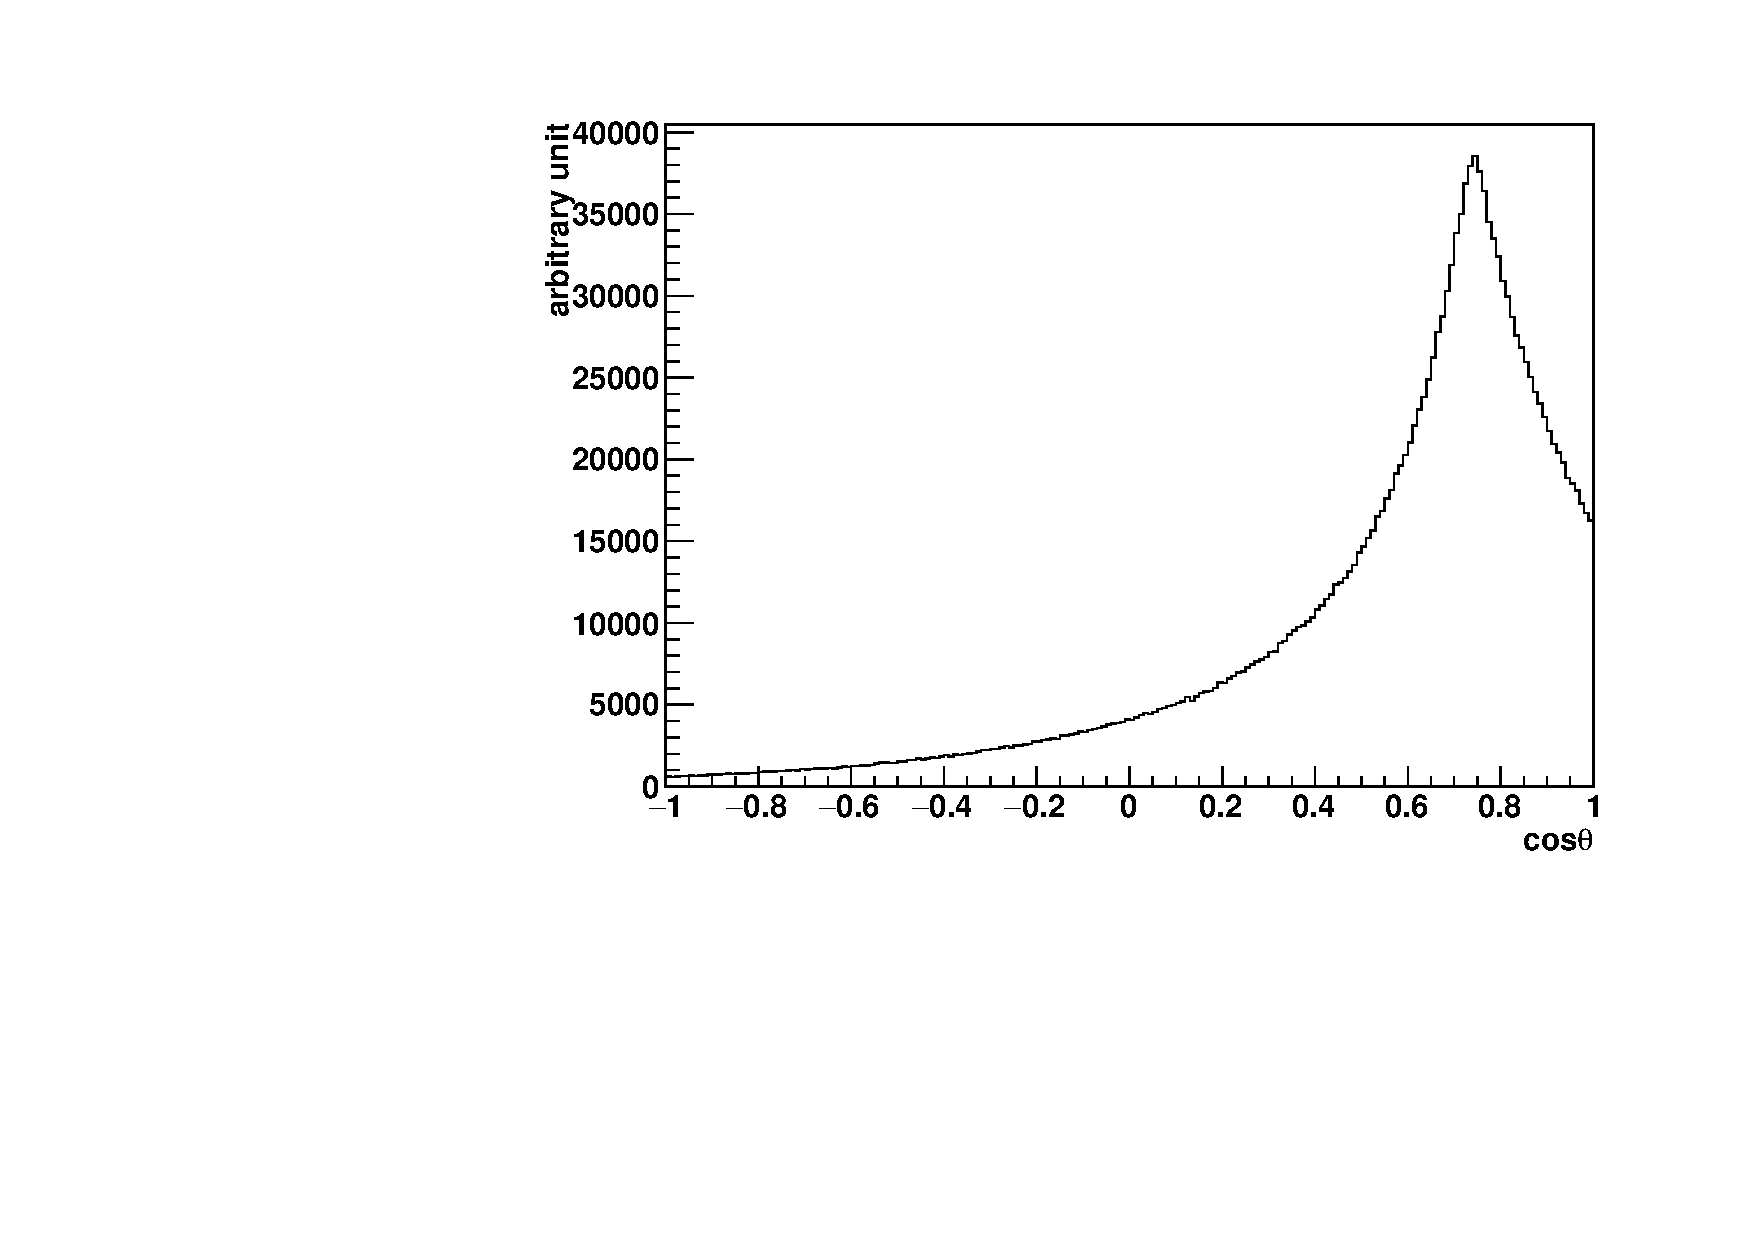
\includegraphics[width=7cm]{ChAngle_pdf.pdf}	
		\end{minipage}	
	}
	\caption{\label{WLS_pdf} The distributions of the pdfs for wbWLS reconstruction. Left: the pdf of the WLS timing spectrum. Right: Angular distribution caused by Cherenkov effect in pure water. It peaked at $\cos\theta_{Ch}\approx 0.75$ ($\theta_{Ch}\approx 41.4^\circ$), which is the same to the water Cherenkov angle $\cos\theta_{Ch}=1/1.33$.}	
\end{figure}

In the wbWLS case, since WLS absorbs and re-emits photons, the above situations are slightly modified to build a WLS fitter.

\begin{figure}[htbp]
	\centering	
	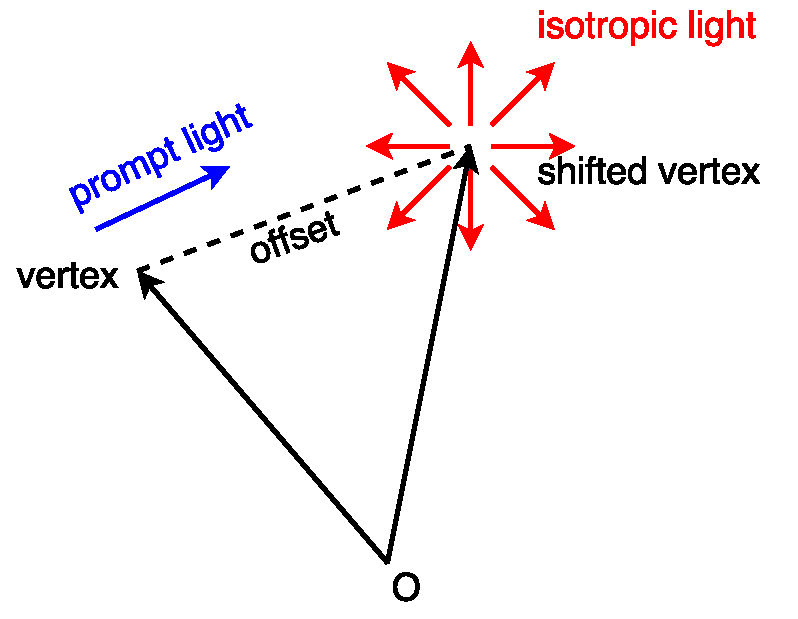
\includegraphics[width=6cm]{FitterDiagram.pdf}
	\caption{\label{FitterDiagram} 
		A diagram shows the shifted position in wbWLS.
	}
\end{figure}

In Fig.~\ref{FitterDiagram}, an event is generated at a vertex, travelling along $\vec n = \vec{p}/|\vec{p}|$ and emitting prompt light. According to the optical property of PPO, this prompt light has a probability of $\sim$0.6 to be absorbed by the WLS and then re-emitted at a shifted vertex along $\vec n$. Then $\overrightarrow{\mathrm{shifted~vertex}}=\overrightarrow{\mathrm{vertex}}+\mathrm{offset}\cdot\vec{n}$.  
The offset we set in the fitter is 100 (mm) obtained from optimization. 

Meanwhile, for the reconstruction of direction, we also need to consider the fraction of the re-emitted and wavelength shifted isotropic light. For this light, the angular distribution for direction is just a flat line, as shown in Fig.~\ref{WLSAngle}.

\begin{figure}[htbp]
	\centering
	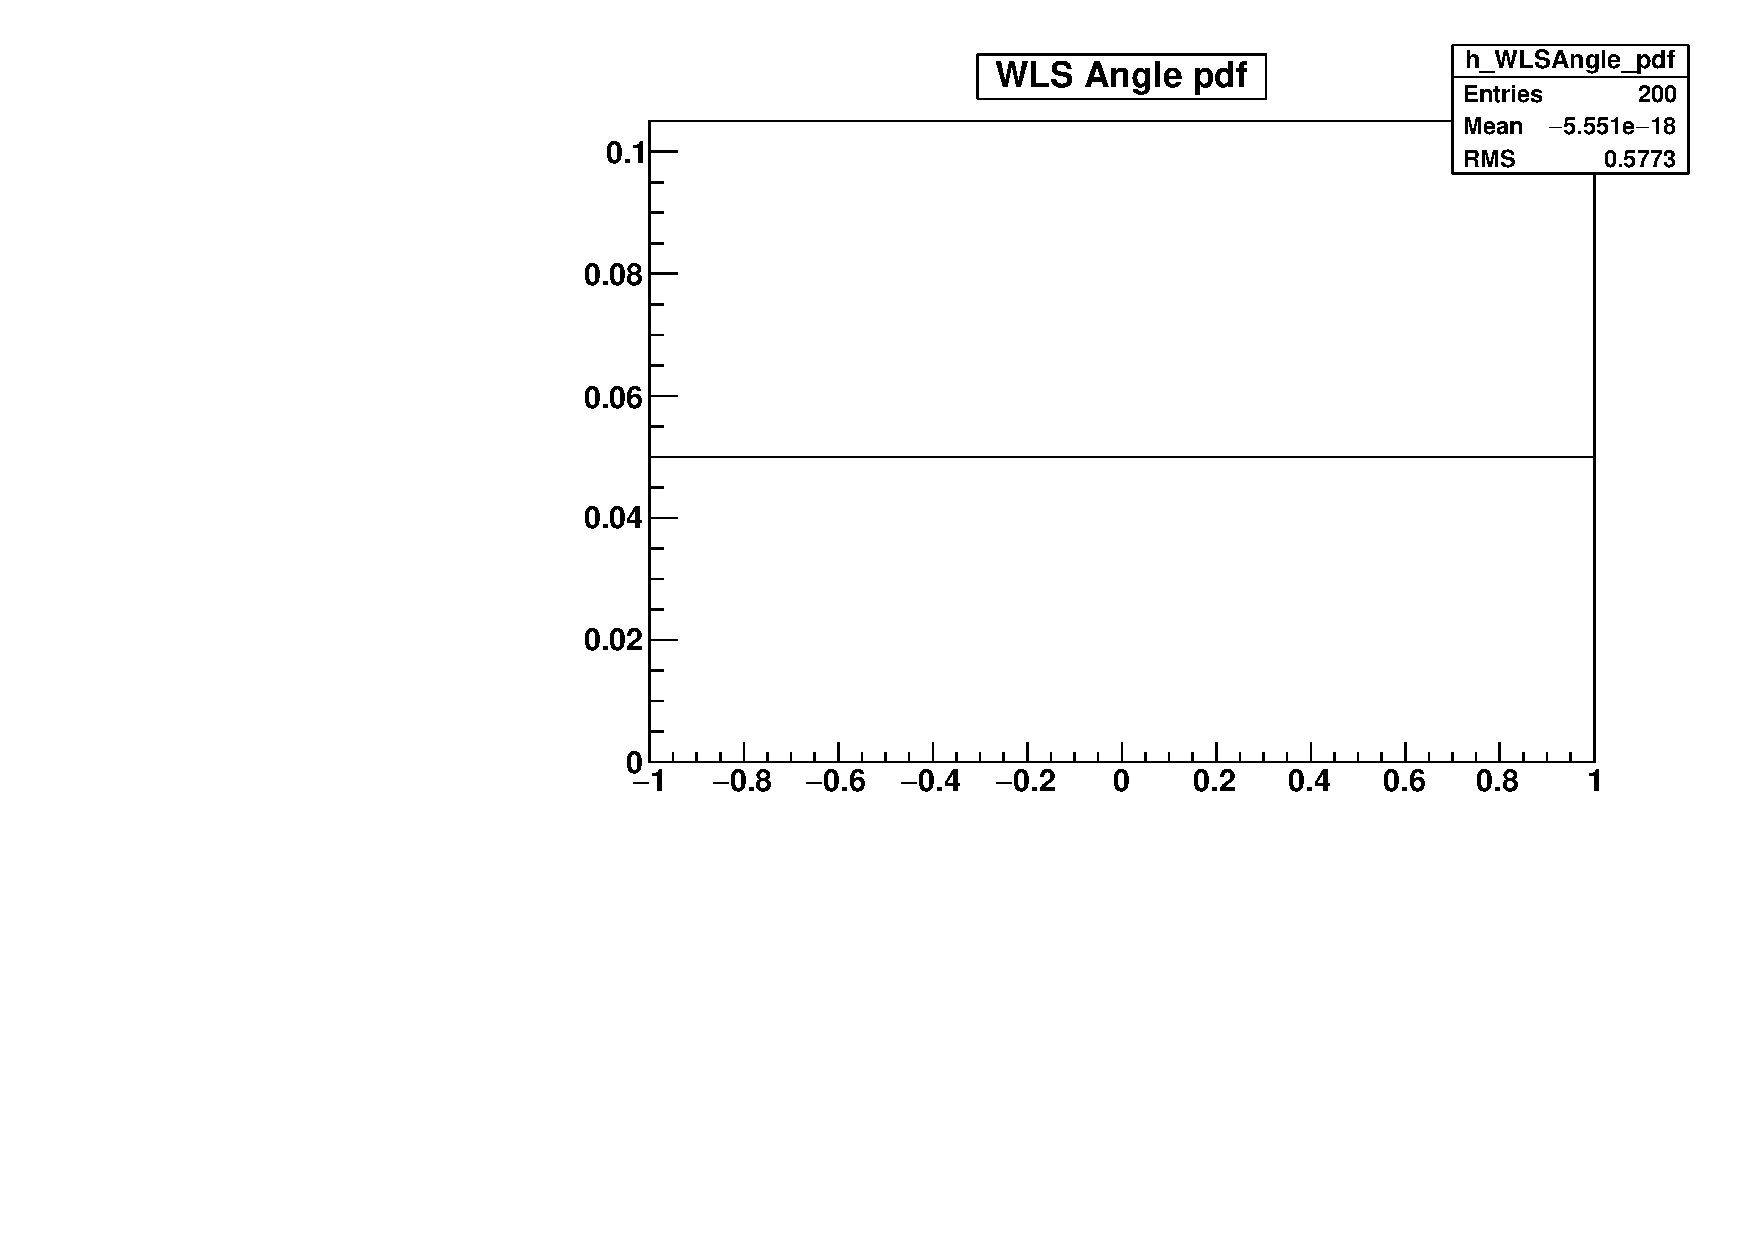
\includegraphics[width=6cm]{WLSAngle_pdf.pdf}
	\caption{Flat angular distribution for re-emitted isotropic light.}
	\label{WLSAngle} 
\end{figure}

To test the WLS fitter performance, 1 to 10 MeV electrons are simulated at the center of the AV filled with wbWLS and travel along +x direction. As a comparison, a same simulation is done for the AV filled with pure water.

Fig.~\ref{WLSFitPos}a shows the performance of the WLS fitter reconstructed positions based on reconstructing the MC simulations. For the fitted position distribution of 5 MeV electrons, we can get a root mean square (RMS) of 200.6 mm and a bias to the center of 29.48 mm. Fig.~\ref{WLSFitPos}b shows that for the 5 MeV electrons in the wbWLS, the RMS of the fitted position is 187.8 mm better than in the pure water.

\begin{figure}[htbp]	
	\centering	
	\subfloat[Simulated electrons from 1 to 10 MeV.]{ 	
		\begin{minipage}[b]{0.5\textwidth}			
			%\centering			
			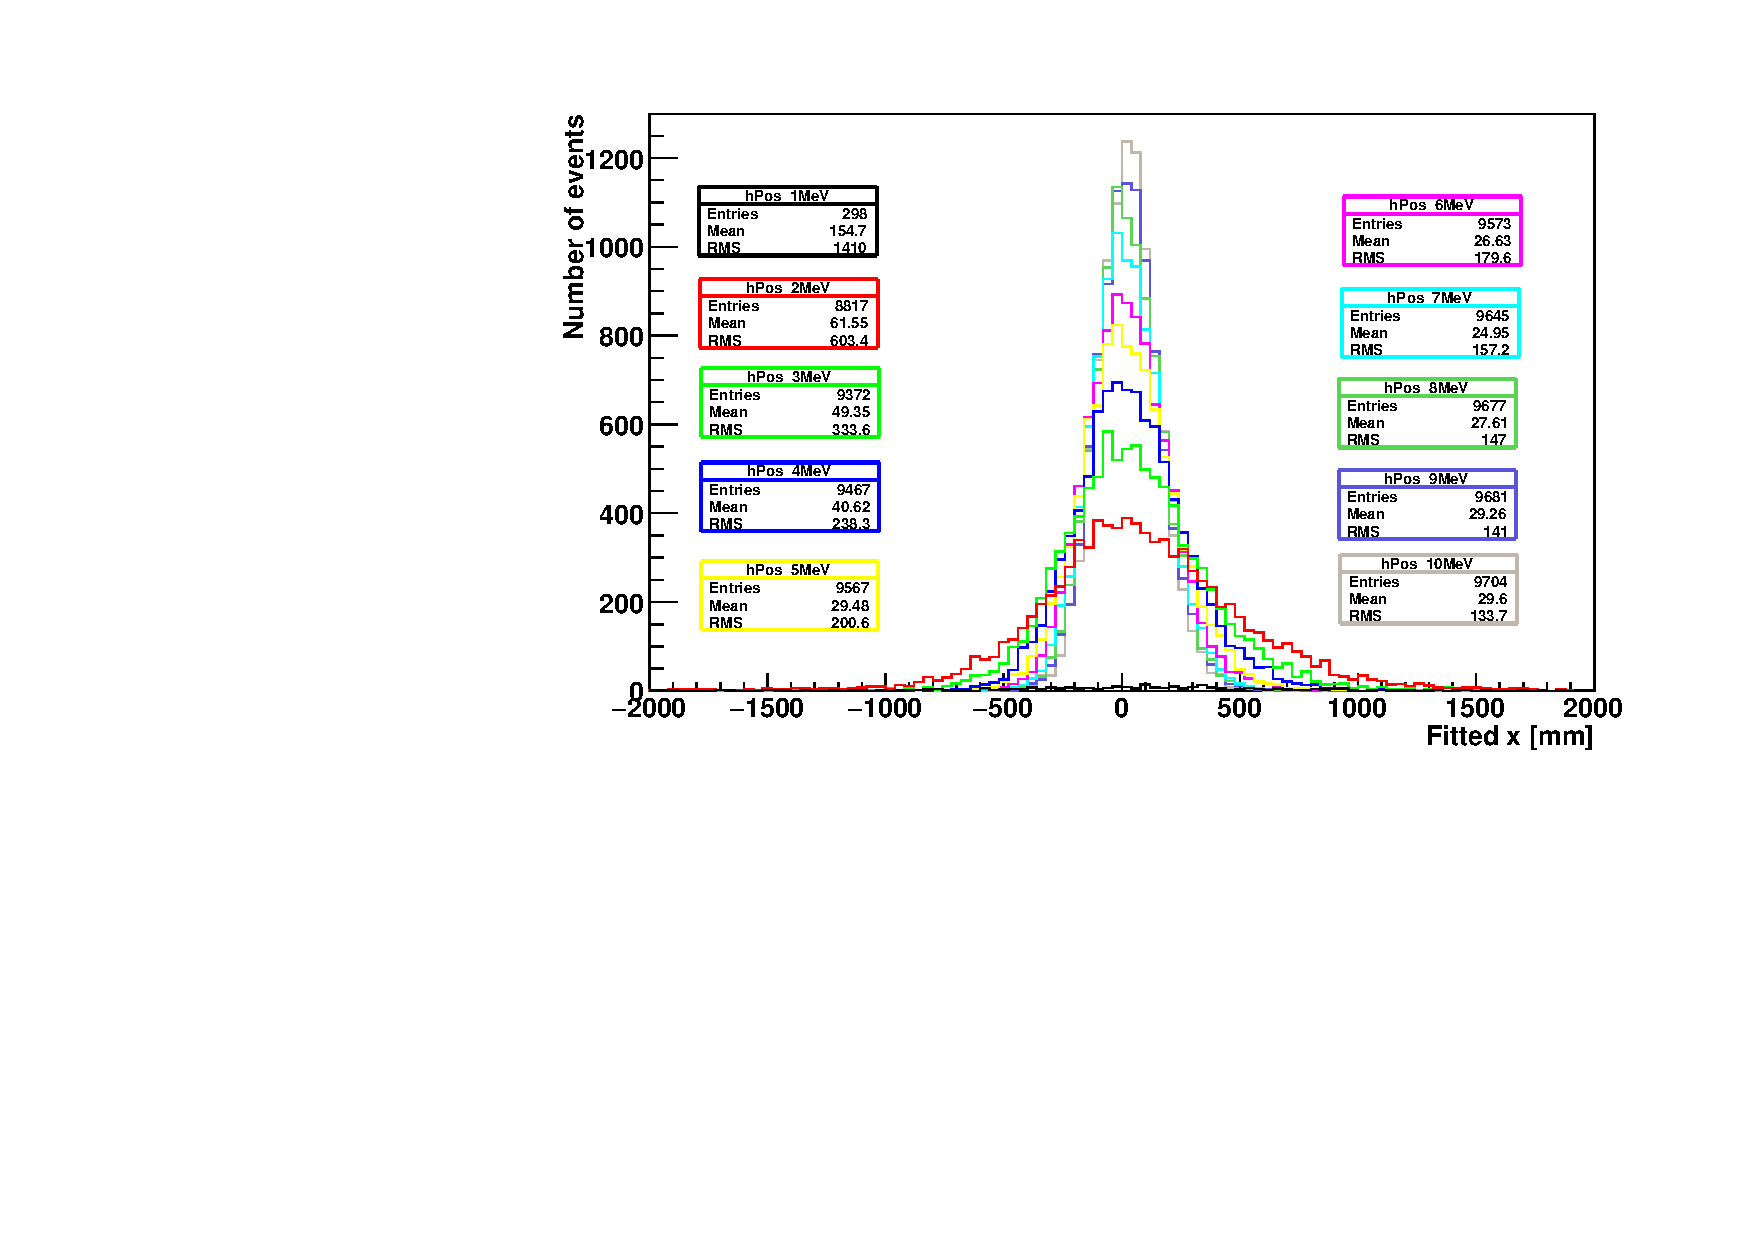
\includegraphics[height=4.5cm]{FittedPPO_Xpos.pdf}	
		\end{minipage}%
	}
	\subfloat[Simulated electrons in the wbWLS or the water.]{		
		\begin{minipage}[b]{0.6\textwidth}		
			%\centering	
			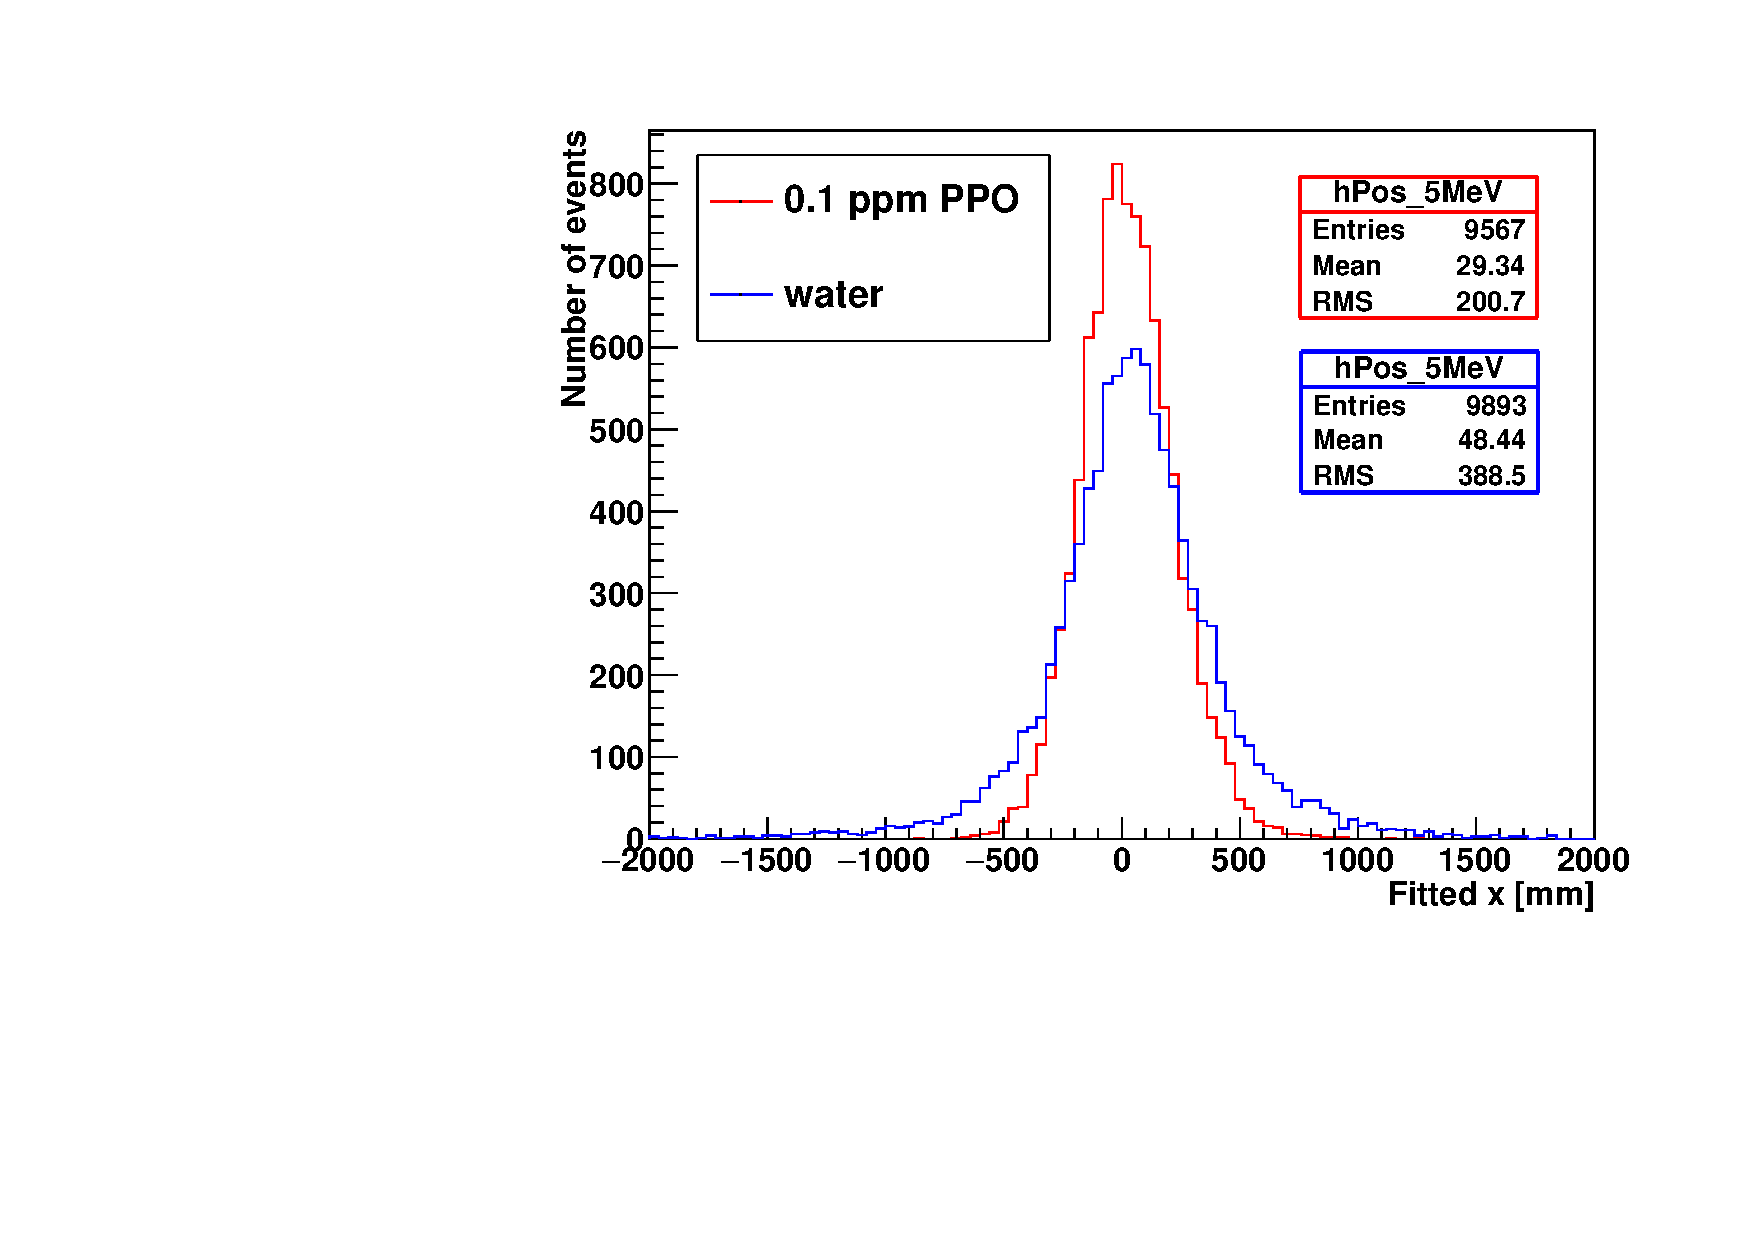
\includegraphics[height=4.5cm]{WLS_FittedPos.pdf}	
		\end{minipage}	
	}	
	\caption{\label{WLSFitPos} Fitted position projected on x axis for: (a) simulated electrons with various energies in the wbWLS. (b) The WLS fitter reconstructed X positions of the 5 MeV electron events in the wbWLS (red) are compared to the ones in the water (blue).
	}
\end{figure}

For a given Cherenkov event, the error in the reconstructed event direction is defined as\cite{boulay}: $\cos(\theta_e)=\vec{u}_{fit}\cdot\vec{u}_e$, where $\vec{u}_e$ is the simulated electron direction and $\vec{u}_{fit}$ is the reconstructed direction. To quantify this error, we define a $\cos\theta_{a}$ so that:
\[
\frac{\int_{\cos\theta_{a}}^1 P(\cos\theta_e) d\cos\theta_e}{\int_0^1 P(\cos\theta_e) d\cos\theta_e} = a
\] 
where $P(\cos\theta_e)$ is the distribution of $\cos\theta_e$ from MC data. $\cos\theta_{a}$ is found numerically to let $\cos\theta_e$ contain $ a\cdot 100\%$ of the reconstructed data. A larger $\cos\theta_{a}$ means a better direction reconstruction.

Table \ref{quantAngular} shows the results of $\cos\theta_{a}$ for SNO heavy water data \cite{boulay}; SNO+ pure water simulation and wbWLS MC. 

\begin{table}[ht]
	\caption{\label{quantAngular}A comparison of quantitative estimates for the angular resolution between the SNO heavy water, SNO+ wbWLS and the SNO+ pure water cases.}	
	{\centering
		\begin{tabular*}{135mm}{c@{\extracolsep{\fill}}cccc}
			\toprule 
			Medium & $\cos\theta_{0.9}$ & $\cos\theta_{0.8}$ & $\cos\theta_{0.5}$
			\\
			\midrule
			SNO heavy water  & 0.50 & 0.71 & 0.92  \\	
			SNO+ water  & 0.53 & 0.76 & 0.93	 \\
			wbWLS  & 0.37 & 0.63 & 0.90  \\	
			\bottomrule	
		\end{tabular*}
	}
\end{table}

To conclude, compared with a pure water SNO+ detector, using a MP-WLS fitter for physics events in wbWLS version of SNO+, we have a better position resolution while the direction is slightly worse but still comparable.

\section{Reconstruction for SNO+ Water Phase}
In the same Multi-path Fitter framework, a fitter for SNO+ pure water phase, the MultiPath Water (MPW) fitter, is developed. 

The MPW fitter scheme is similar to the WLS fitter but without considering the WLS effects. Fig.~\ref{mpwpdf} shows the timing pdf for position reconstruction and the angular pdf for direction reconstruction. In the left panel of Fig.~\ref{mpwpdf}, the timing pdf is the measured PMT response time distribution from SNO time, tuned by the $^{16}$N calibration data for SNO+ water phase. The early and late light response are forced to be de-weighted by assigning straight lines. In the right panel of Fig.~\ref{mpwpdf}, the angular pdf is extracted from the MC simulation, which is the same to the Fig.~\ref{WLS_pdf}b.

\begin{figure}[htbp]
	\centering
	\begin{minipage}[t]{0.48\textwidth}
		\centering
		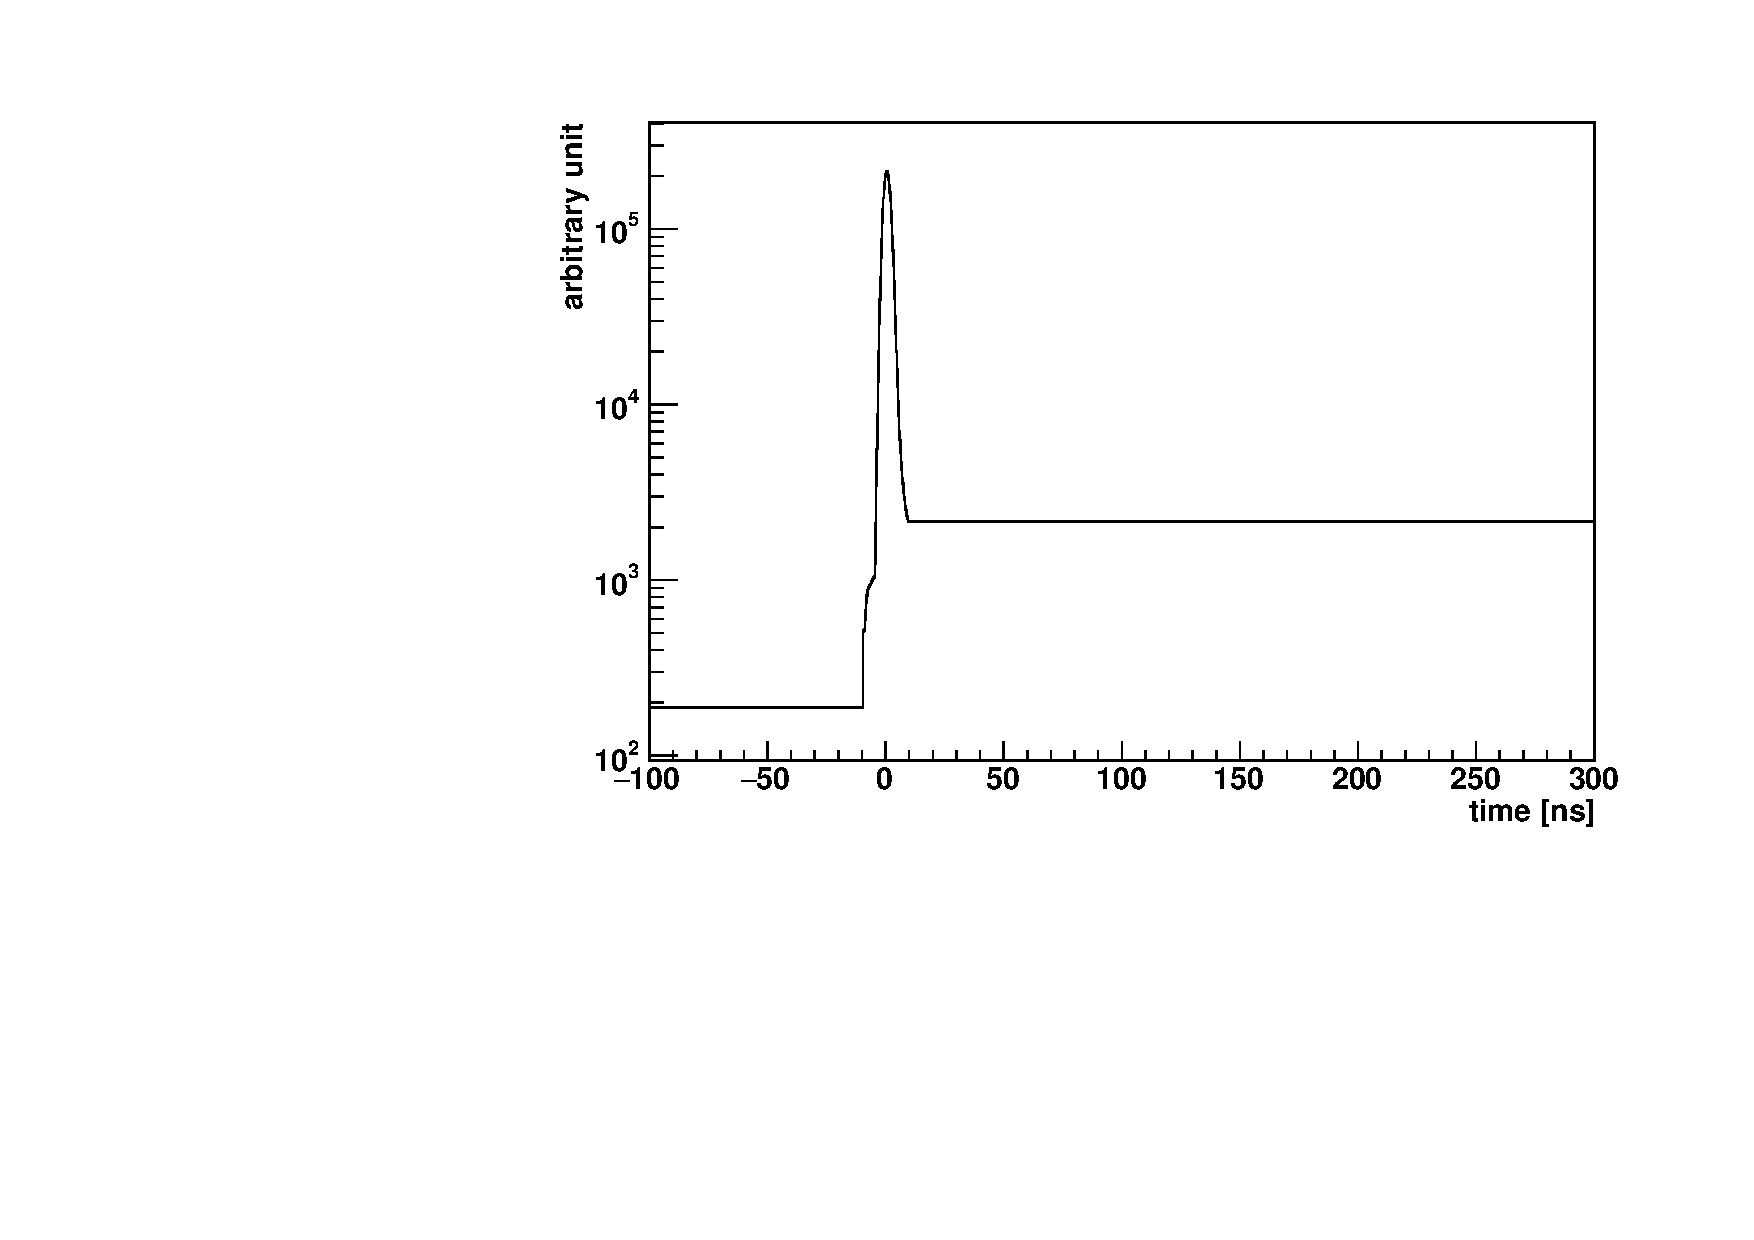
\includegraphics[width=7cm]{MPW_timingPDF.pdf}
	\end{minipage}
	\begin{minipage}[t]{0.48\textwidth}
		\centering
		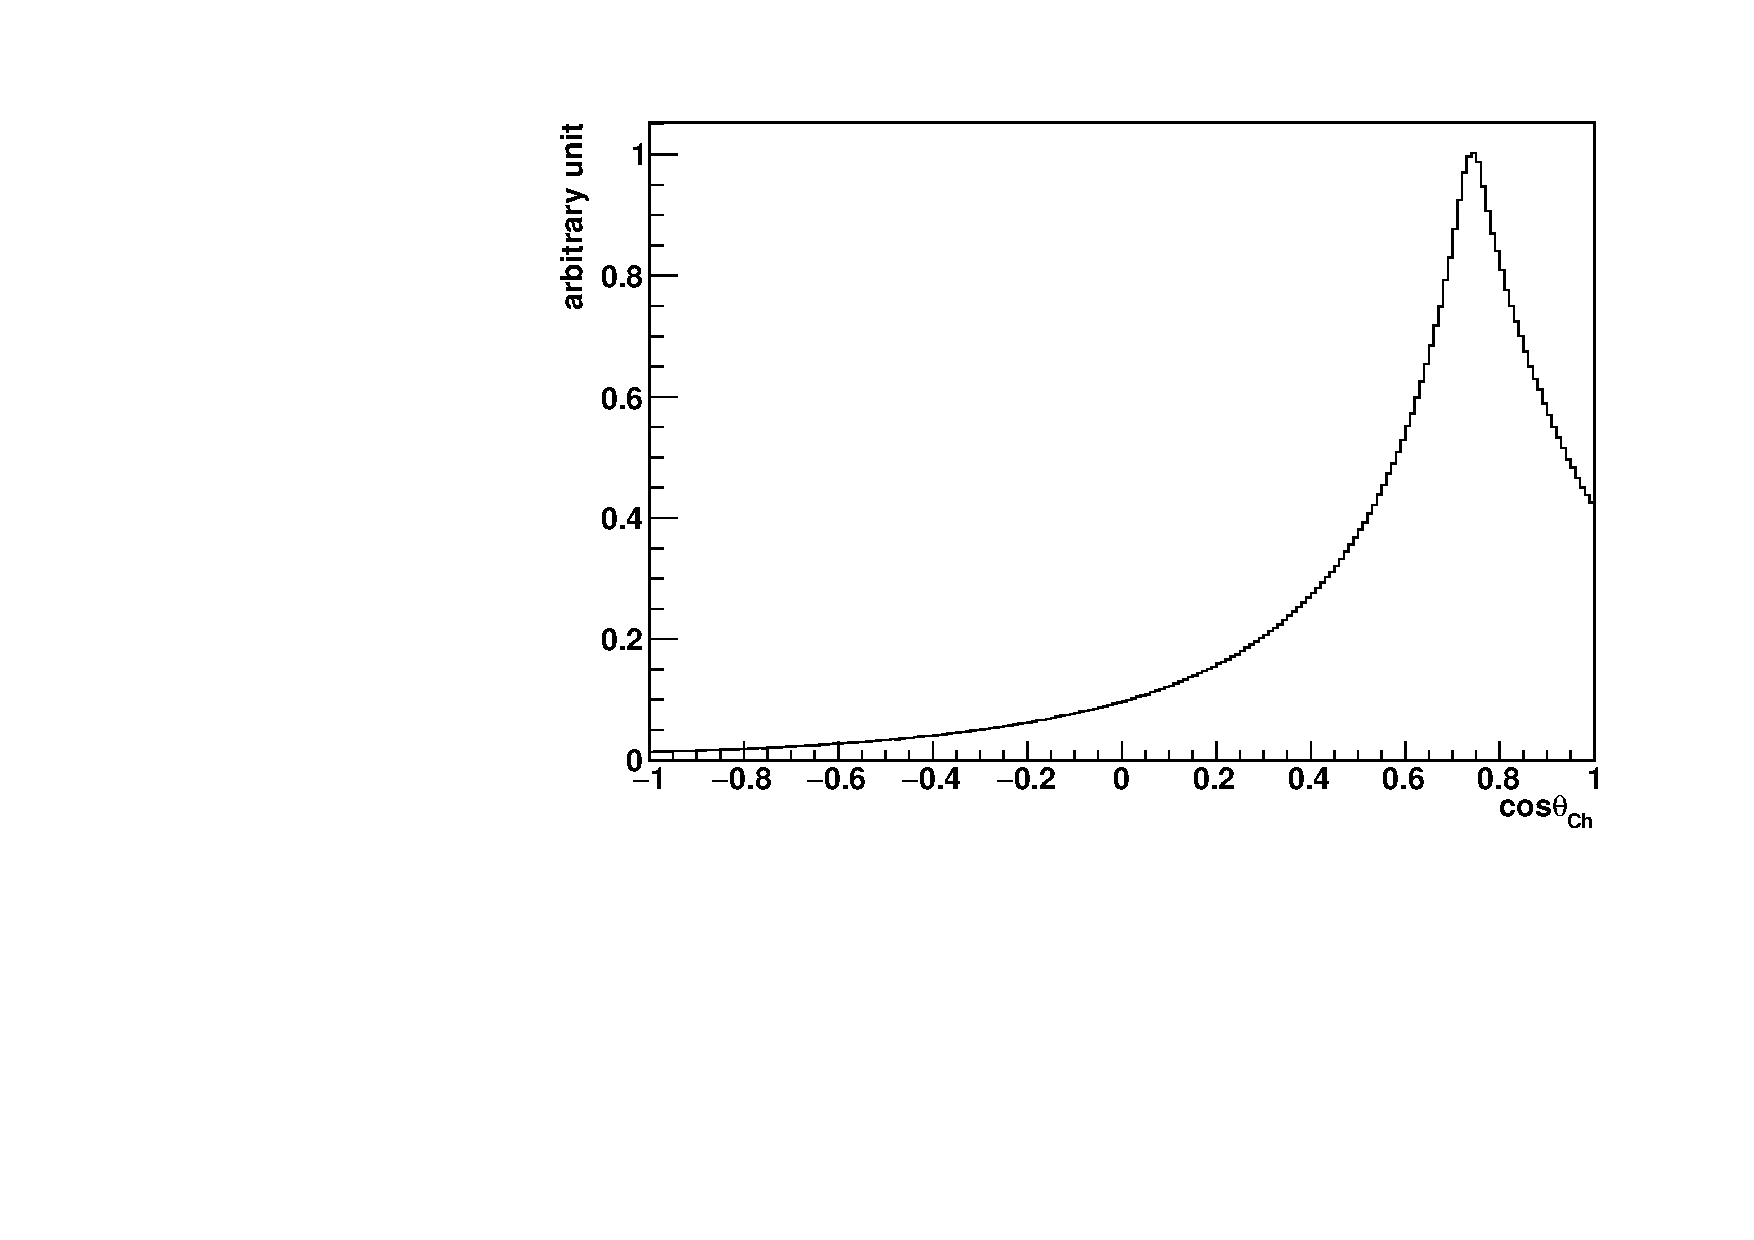
\includegraphics[width=7cm]{MPW_angularPDF.pdf}
	\end{minipage}
	\caption{Pdfs for the MPW fitter reconstruction. Left: PMT response time tuned by calibration data as the timing pdf. Right: PMT angular distribution as the angular response pdf.}
    \label{mpwpdf}
\end{figure}

\section{Testing the MPW Fitter with SNO+ $^{16}$N Calibration}
The SNO+ detector is currently filled with water and has been under water phase operation for almost a year. In order to calibrate the detector, an Nitrogen-16 ($^{16}$N) calibration source inherited from the SNO experiment was deployed for calibration scans in June and November, 2017 and March, 2018. 

The $^{16}$N calibration runs provide an ideal test for the fitter performances. From a comparison of reconstructions for data and MC, we can also extract systematics of the MPW fitter reconstruction. 

\subsection{Fitter Performances}

The $\gamma$ rays emitted from the $^{16}$N source interact with the water in the detector and the electrons are generated. Fig.~\ref{hsx} shows the x distributions of the first $\gamma$-ray interaction points (spatial distribution S(x)) obtained from MC simulation.

\begin{figure}[!htb]
	\centering
	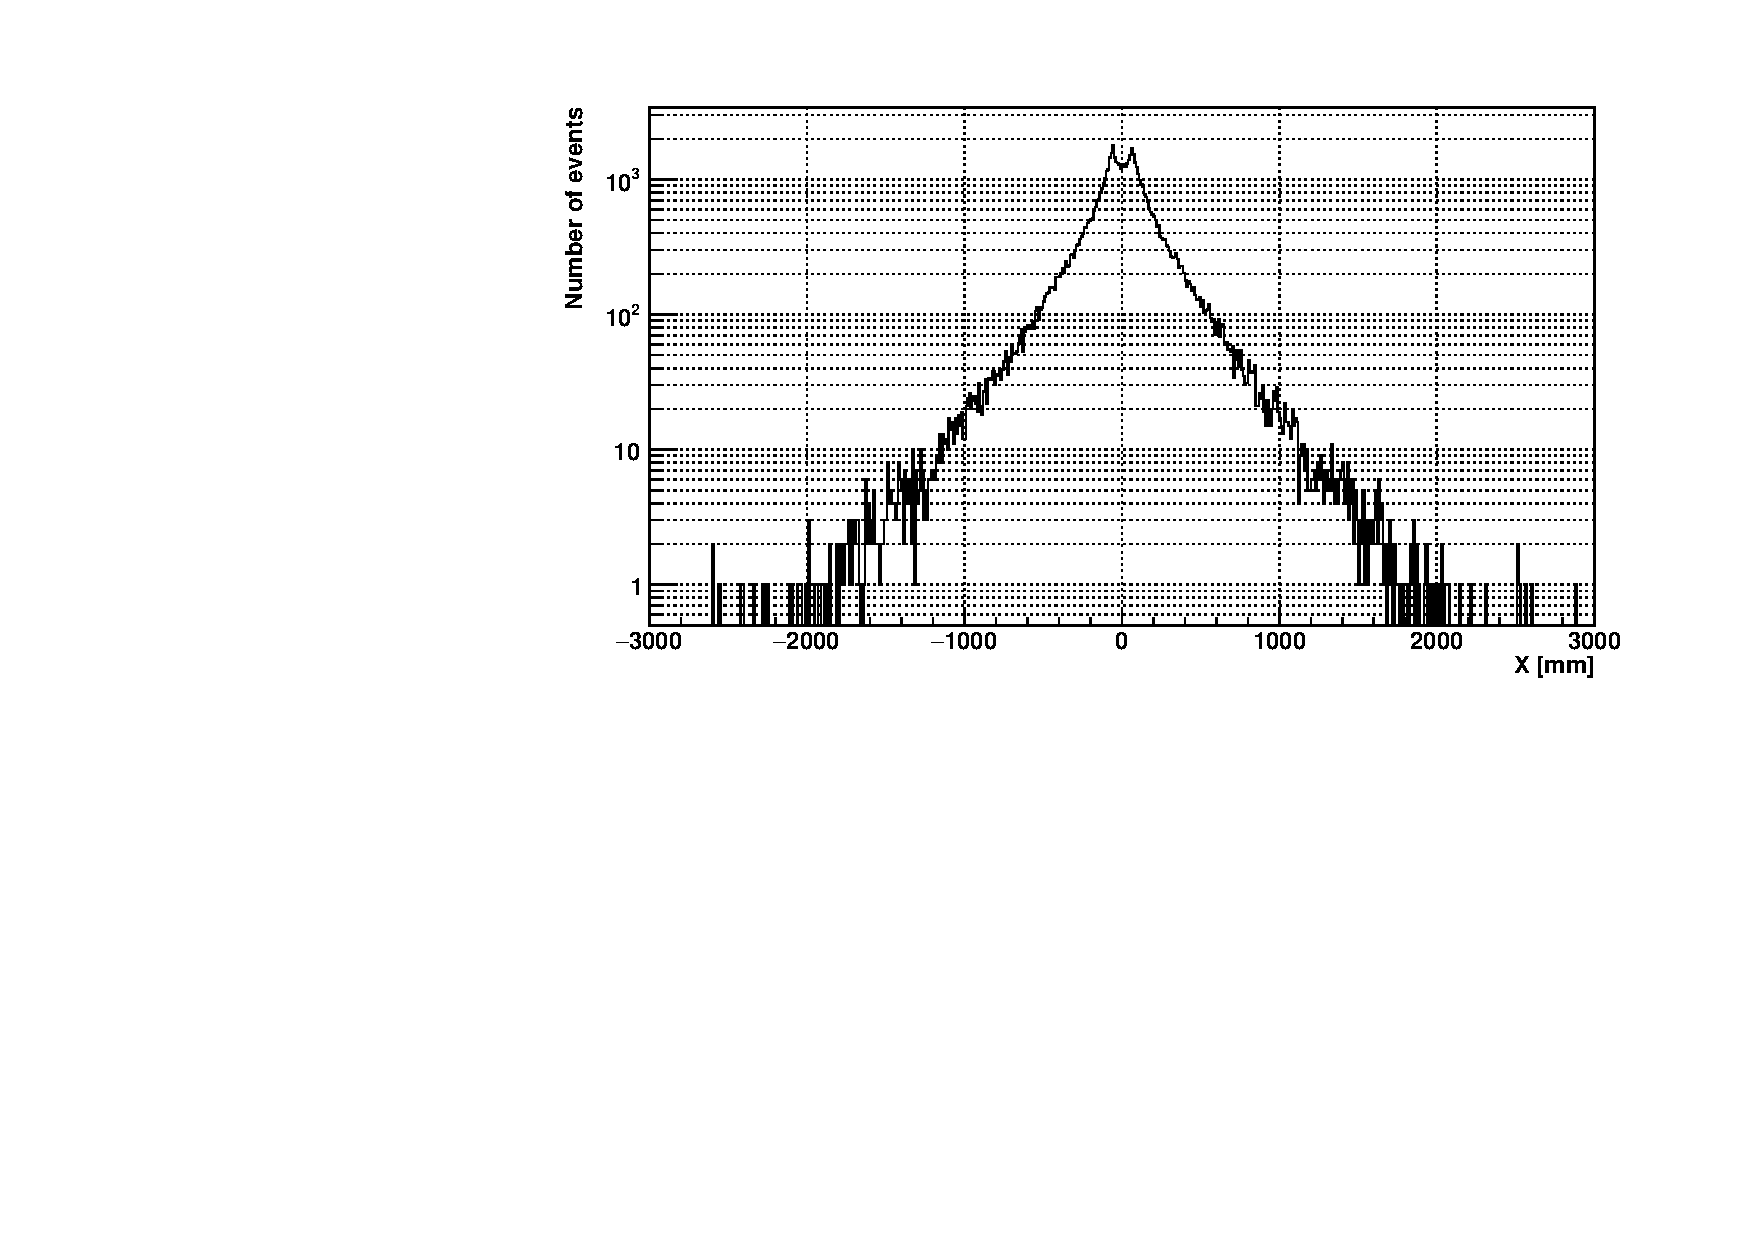
\includegraphics[width=8cm]{sx.pdf}
	\caption{Distributions of {$^{16}$}N first $\gamma$-rays interaction position projected on x axis, obtained from simulations.}
	\label{hsx}
\end{figure}

A position resolution function is defined for the fitted electron position distribution\cite{boulay}:
\[
  R(x)=\frac{1-\alpha_e}{\sqrt{2\pi}\sigma_p}\exp{[-\frac{1}{2}(\frac{x-\mu_p}{\sigma_p})^2]+\frac{\alpha_e}{2\tau_p}\exp{[\frac{-|x-\mu_p|}{\tau_p}]}}
\]
where: $\alpha_e$ = the fractional exponential component, $\sigma_p$ =
the Gaussian width, $\mu_p$ = the Gaussian shift, $\tau_p$ = the
exponential slope.

For electrons from the $^{16}$N calibration source, the position resolution function is smeared by the convolution of S(x) as:
\[
  N_{R}=\frac{dN}{dx_R}=\int^\infty_\infty S(x)R(x_{fit}-x)dx
\]

A $\chi^2$ can be calculated as
\[
  \chi^2=\sum^{N_{bins}}_{i=0}[\frac{N_R(x_{fit}^i)-N_{fit}(x_{fit}^i)}{\sigma_i}]^2
\]
where
\[N_R(x_{fit}^i)=\sum_{x_i=-\infty}^{+\infty}S(x_i)R(x_{fit}^i-x_i)\]

By minimizing the $\chi^2$, the parameters of the resolution function, $\{\alpha_e,\mu_p,\sigma_p,\tau_p\}$ are obtained.

Fig.~\ref{posresol} shows the MPW fitter reconstructed x position of {$^{16}$}N events from data and MC. The reconstructed position distributions are fitted with $N_R(x_{fit})$.

\begin{figure}[!htb]
	\centering
	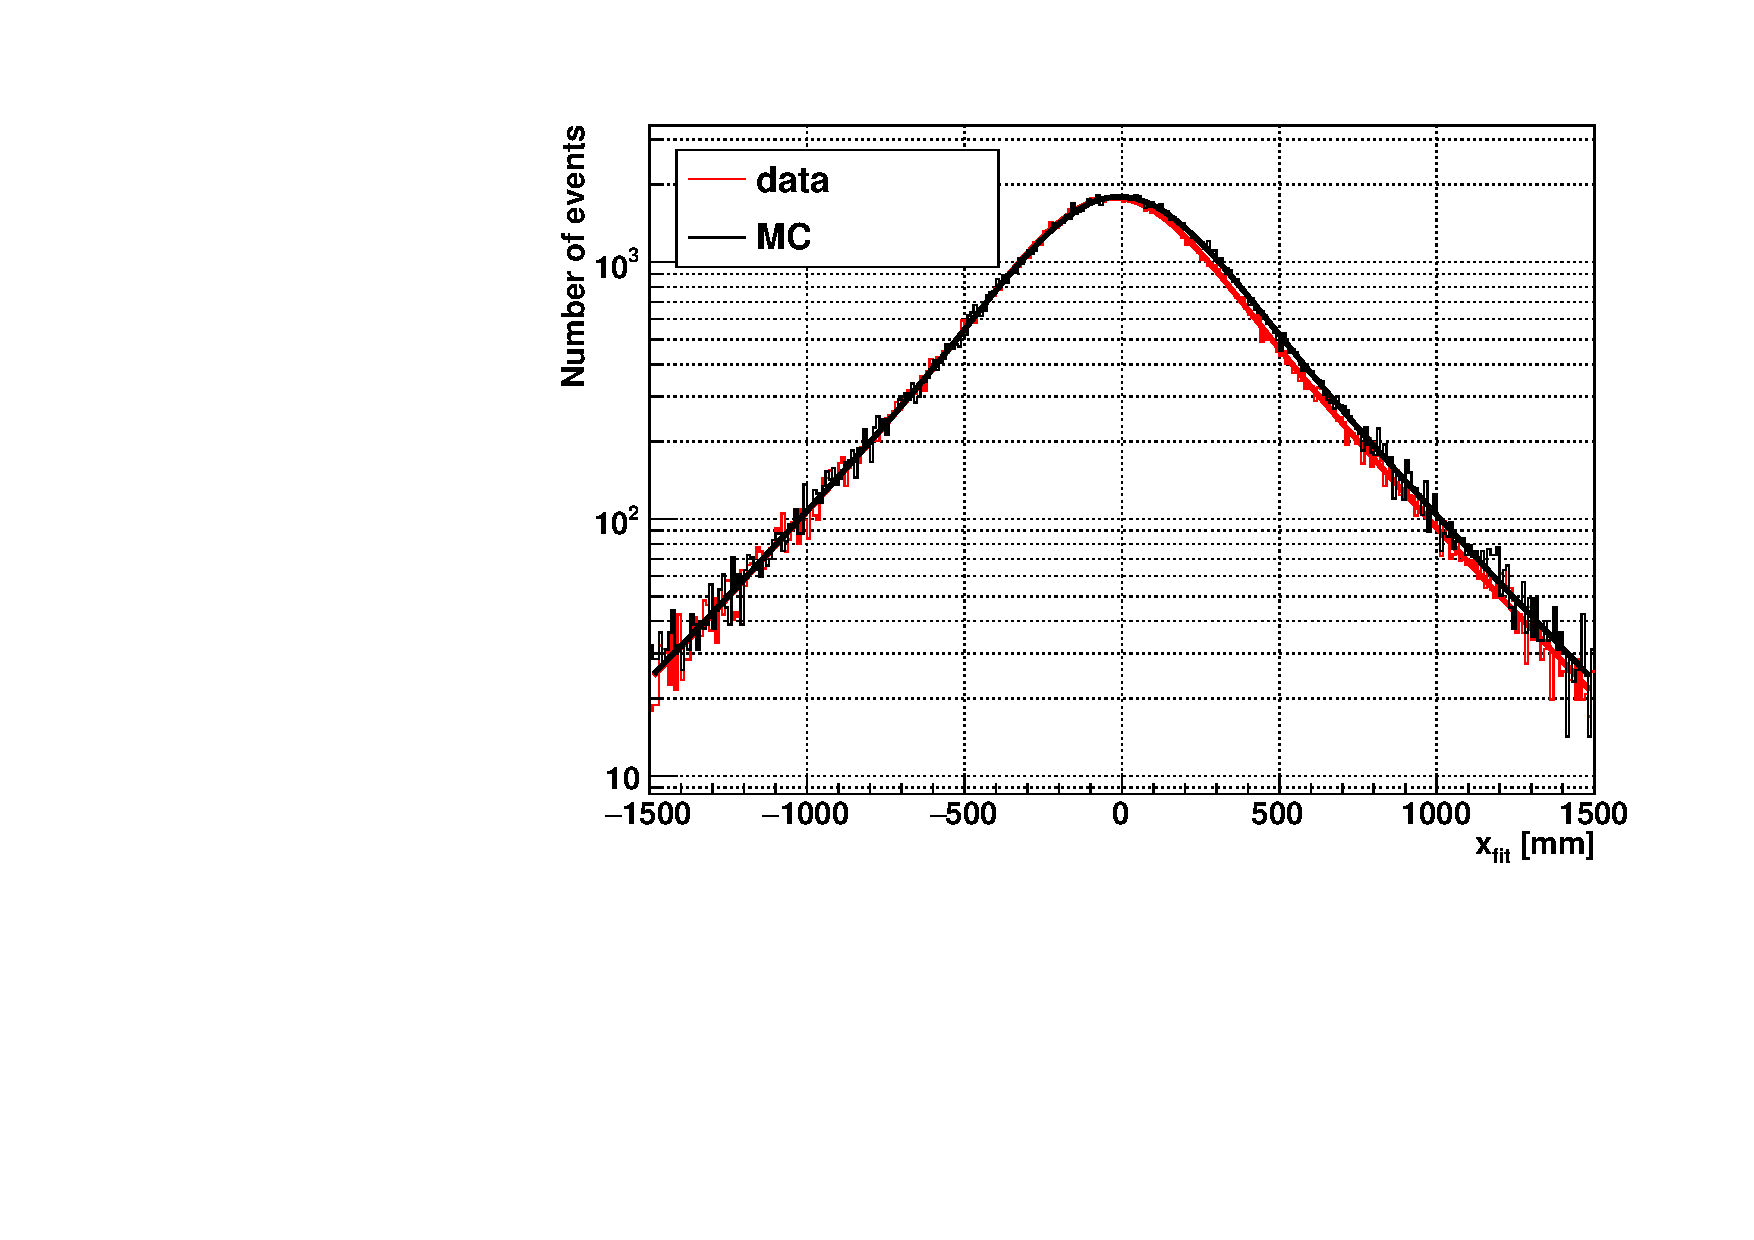
\includegraphics[width=10cm]{posResol.pdf}
	\caption{Distributions of the reconstructed position projected on x axis, obtained from SNO+ {$^{16}$}N central run data (red) and MC (black). The distributions are fitted with $N_R$, the position resolution function convolved with the distribution of the first $\gamma$ interaction positions.}
	\label{posresol}
\end{figure}

Table.~\ref{table_posresol} summarizes the values of position biases and resolutions obtained from data and MC of SNO+ {$^{16}$}N runs at the detector center.
\vspace{2mm}
\begin{table}[ht]
\centering
\caption{Position resolution parameters for the MPW fitter. Unit: mm.}
\label{table_posresol}
\begin{tabular}{|p{2.5cm}|p{2.2cm}|p{2.1cm}|p{2.1cm}|p{2.1cm}| p{2.1cm}|}
\hline
MPW fitter & $\alpha_e$ & $\sigma_P$ &  $\tau_P$ &  $\mu_P$\\
\hline 
data& 0.58$\pm$0.04 & 175.8$\pm$3.8 & 288.0$\pm$5.7 & -28.8$\pm$1.0\\	
\hline 
MC & 0.51$\pm$0.05 & 195.2$\pm$3.3 & 298.4$\pm$6.1 & -10.9$\pm$1.0\\
\hline
\end{tabular}
\end{table}

\vspace{5mm}

For the $^{16}$N events, the direction resolutions are obtained from the distribution of $\cos\theta_e$. The $\cos\theta_e$ is defined as:
\[
\cos\theta_e = \vec{u}_{fit}\cdot (\vec{X}_{fit}-\vec{X}_\mathrm{source})/|\vec{X}_{fit}-\vec{X}_\mathrm{source}|
\]
where $\vec{u}_{fit}$ = reconstructed direction, $\vec{X}_{fit}$ = reconstructed position and $\vec{X}_\mathrm{source}$ = true source position. Here $(\vec{X}_{fit}-\vec{X}_\mathrm{source})/|\vec{X}_{fit}-\vec{X}_\mathrm{source}|$ with $|\vec{X}_{fit}-\vec{X}_\mathrm{source}|>1.5~m$ is considered as the true event direction.

The distribution of the $\cos\theta_e$ is described by the angular resolution function\cite{boulay}:
\begin{equation}
P(\cos\theta_e)=\alpha_M\frac{\beta_M\exp[\beta_M(\cos\theta_e-1)]}{1-\exp(-2\beta_M)}+(1-\alpha_M)\frac{\beta_S\exp[\beta_S(\cos\theta_e-1)]}{1-\exp(-2\beta_S)}
\end{equation}

\begin{figure}[!htb]
	\centering
	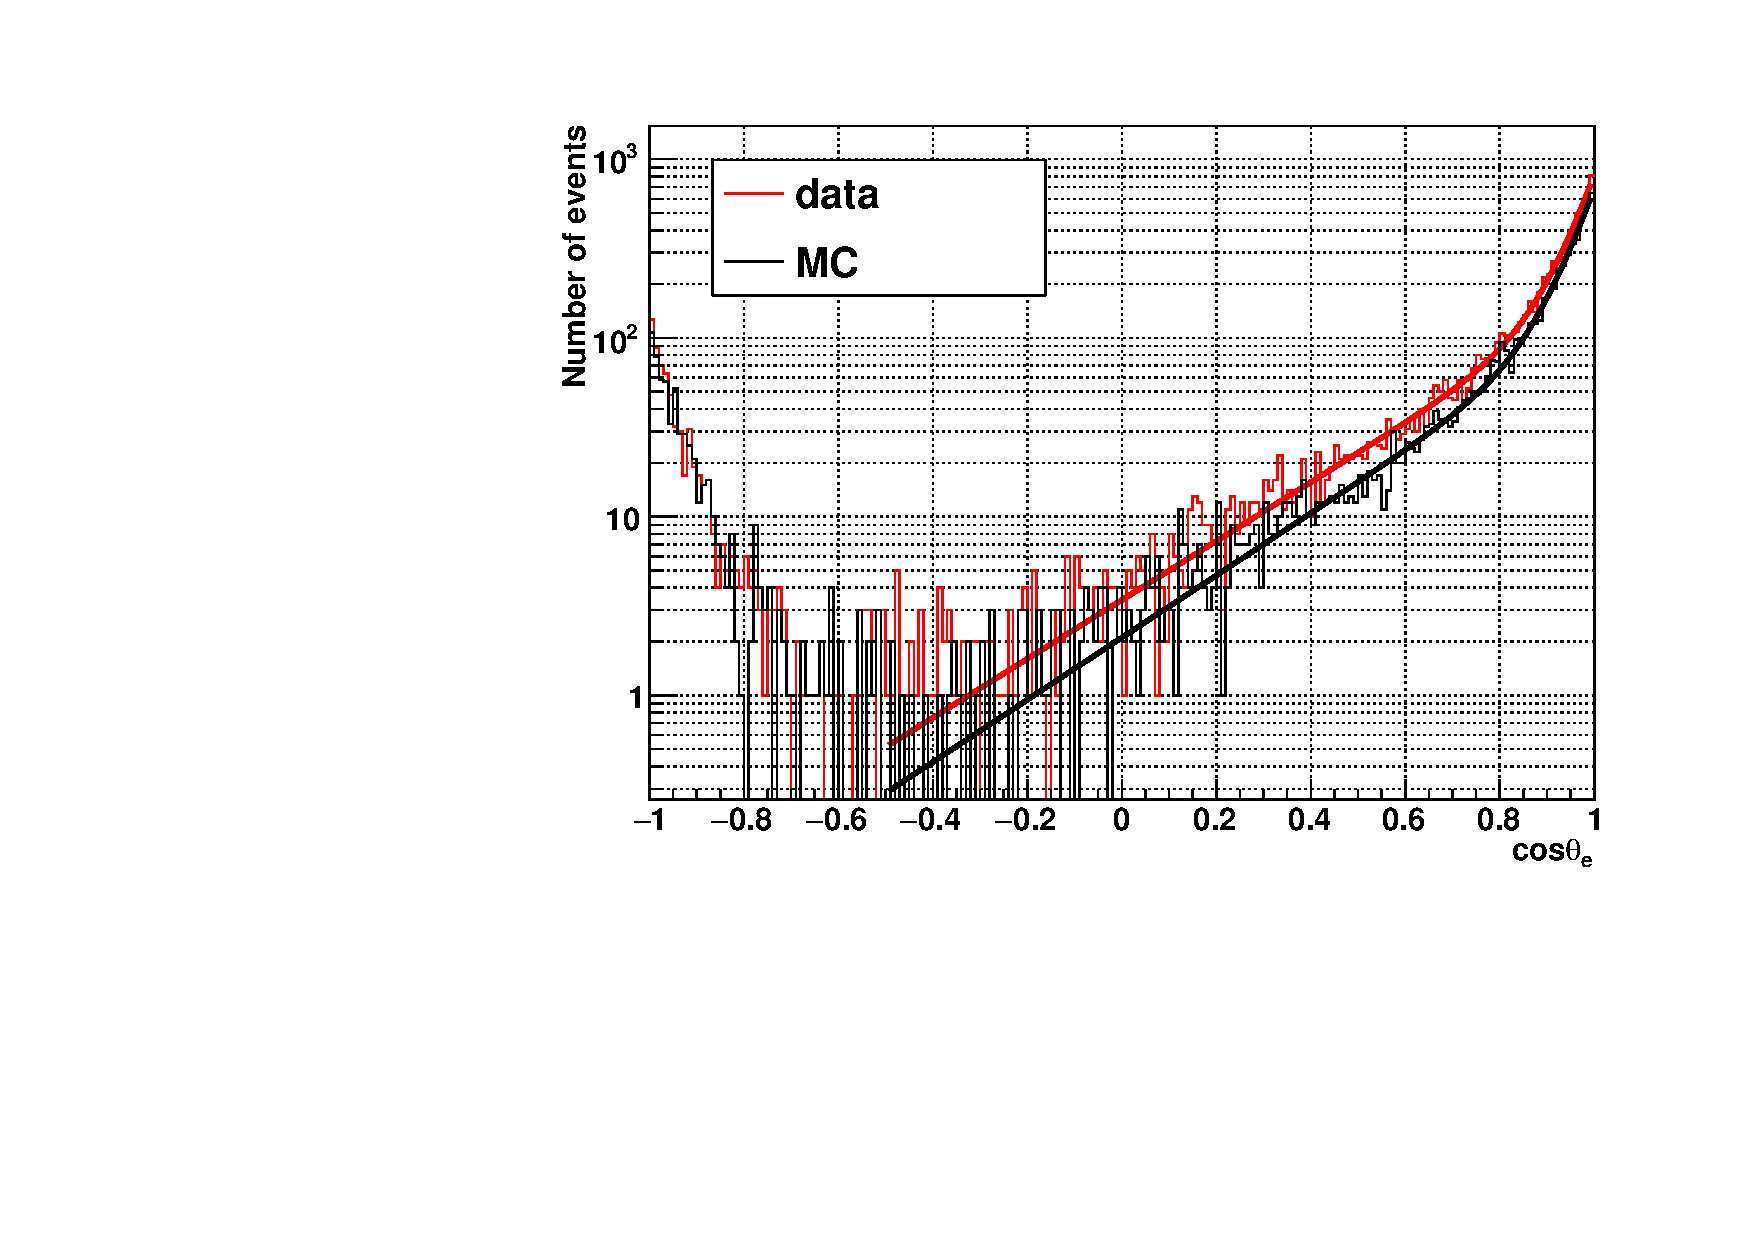
\includegraphics[width=10cm]{angularResol.pdf}
	\caption{Angular resolution distributions obtained from SNO+ {$^{16}$}N runs at the detector center. Red: data; black: MC. The distributions are fitted with angular resolution function.}
	\label{angularesol}
\end{figure}

Table.~\ref{directResol} summarizes the values of direction resolutions. $\cos\theta_a$ values are also listed for showing the fitter performances.

\begin{table}[ht]
	\centering
	\caption{Direction resolution parameters for the MPW fitter.}
	\label{directResol}
\begin{tabular}{|p{2.2cm}|p{1.8cm}|p{2cm}|p{2cm}|p{1.1cm}|p{1.1cm}|p{1.1cm}| }
\hline
MPW fitter& $\beta_M$ &  $\beta_S$ & $\alpha_M$ & $\cos\theta_{0.5}$ & $\cos\theta_{0.8}$& $\cos\theta_{0.9}$\\
\hline
data & 3.79$\pm$0.12 & 18.58$\pm$0.95 & 0.53$\pm$0.02& 0.982 & 0.743 & 0.379\\
\hline
MC &4.01$\pm$0.19 & 18.41$\pm$1.06 & 0.48$\pm$0.03 & 1 & 0.779 & 0.433  \\
\hline
\end{tabular}
\end{table}

\section{SNO+ Partial-fill Reconstruction}
\subsection{MultiPath Partial Fitter}
In the same MP fitter framework, a MP partial fitter is developed for SNO+ partial-fill position and time reconstruction.

In the partial fill geometry, photons will travel with different speeds as they pass through two different mediums, water and scintillator. Assuming a straight light path, the MP partial fitter mainly calculates the total length of the light path ($|\vec{l}_p|=|\vec{X}_{PMT}-\vec{X}_{vertex}|$) and separates it into the lengths in scintillator ($d_{sp}$) and in water ($|\vec{l}_p|-d_{sp}$).

\begin{figure}[!htb]
	\centering
	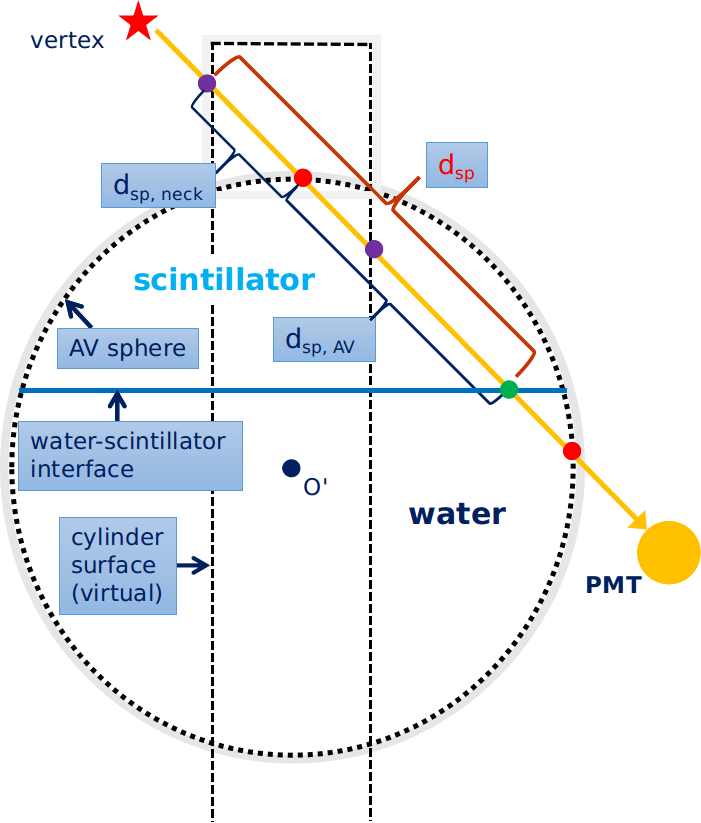
\includegraphics[width=6cm]{scintpath.png}
	\caption{Light path calculation for partial fitter.}
	\label{scintpath}
\end{figure}

As illustrated in Fig.~\ref{scintpath}, a detailed calculation of $d_{sp}$ includes evaluations of (1) light path and neck (line-cylinder) intersection; (2) light path and AV sphere (line-sphere) intersection and (3) light path and water-scintillator interface (line-plane) intersection. $d_{sp}$ is further separated into the path length in neck ($d_{sp,neck}$) and in AV ($d_{sp,AV}$).

Then the time of flight is obtained by:
\begin{equation}
tof = \frac{|\vec{l}_p|-d_{sp}}{v_{gr,water}} +\frac{d_{sp}}{v_{gr,scint}}
\end{equation}
Then the time residue is found:
\begin{equation}
t_{res} = t_{PMT}-tof-t_0
\end{equation}

\begin{figure}[htbp]
	\centering	
	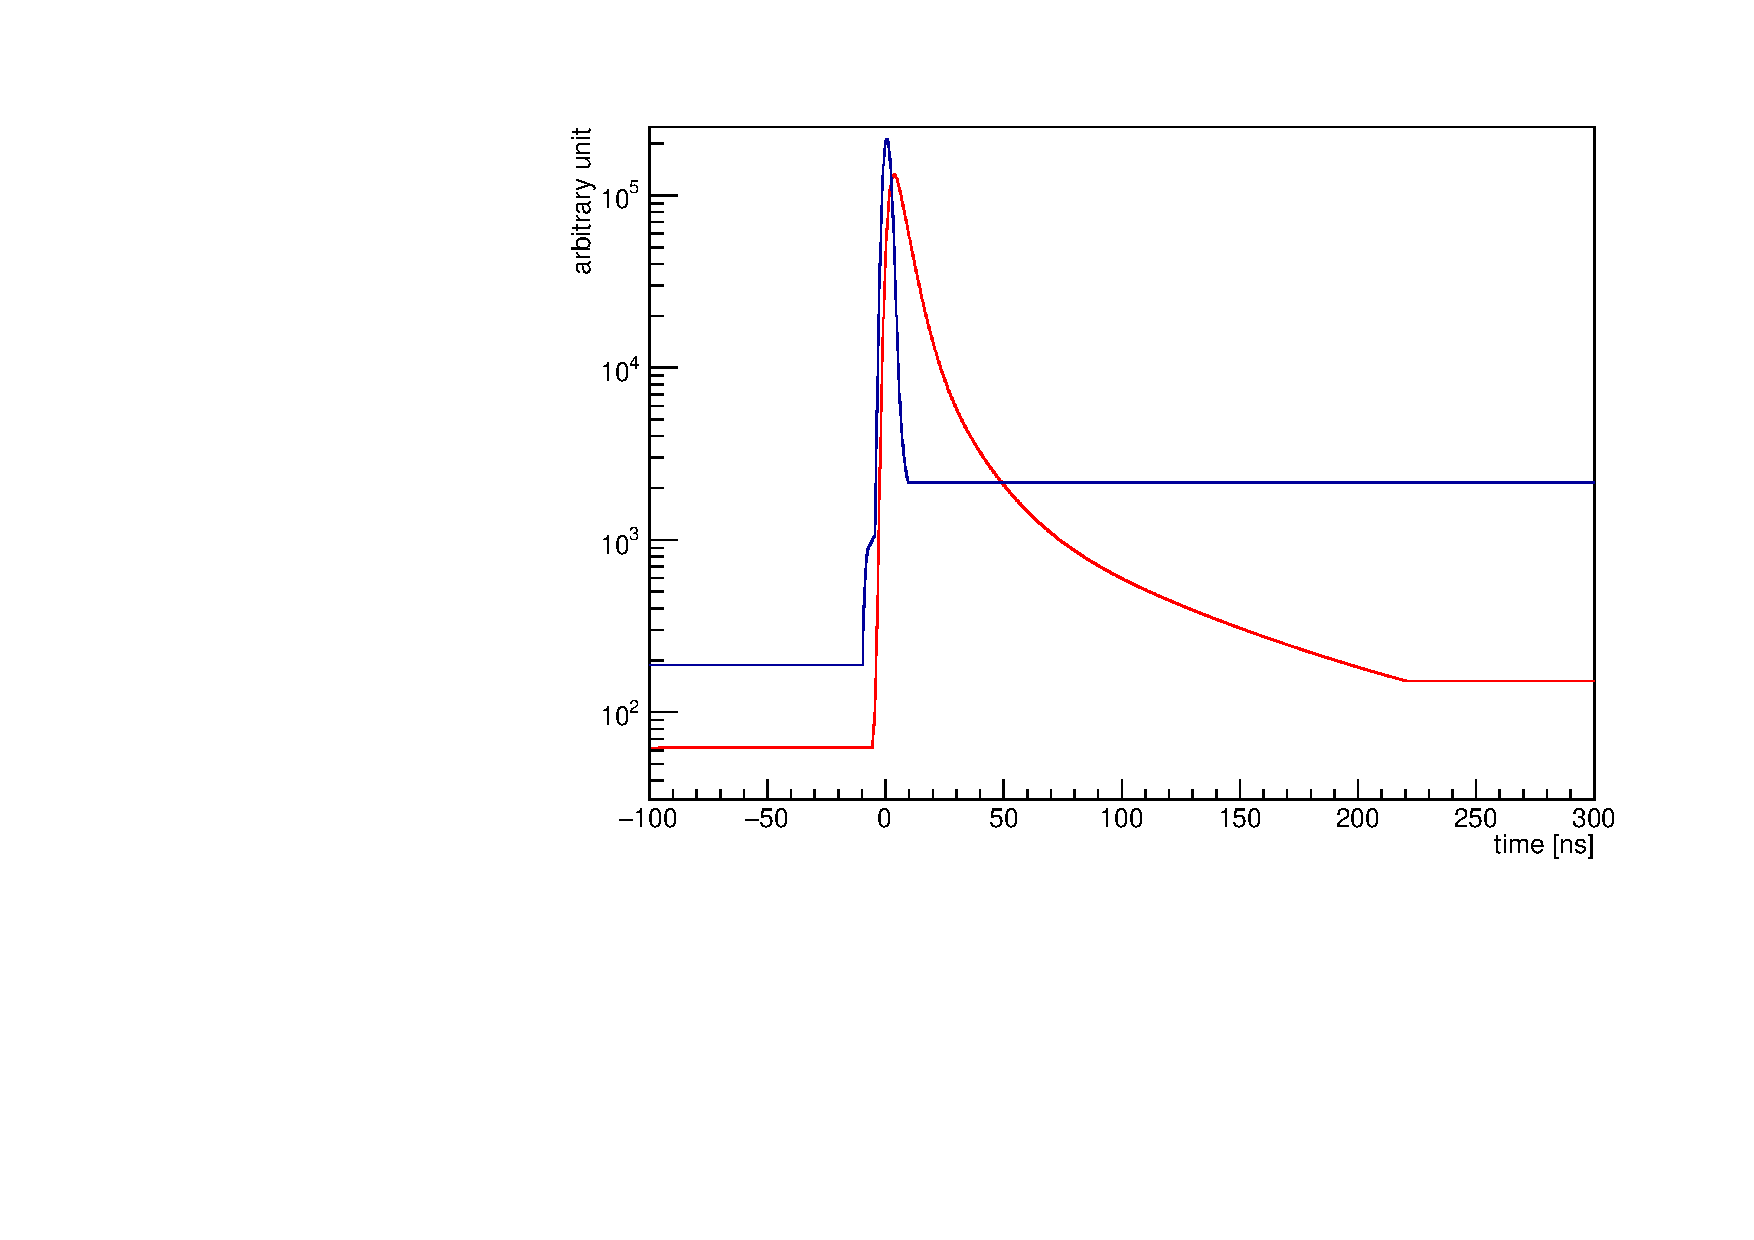
\includegraphics[width=8cm]{scintpdf.pdf}
	\caption{ Pdfs used by MP partial fitter. Blue: the timing pdf used by the MPW fitter; Red: the scintillator timing pdf.}
	\label{partialpdf}
\end{figure}

If $d_{sp}=0$, the light path is always in the water. In this case, the fitter is the same as the MPW. The fitter fits with the MPW pdf. Once the light path passes through the scintillator region, the fitter fits with a scintillator timing pdf, as shown in Fig.~\ref{partialpdf}.

\begin{figure}[htbp]
	\centering
	\subfloat[scintillator region]{
		\begin{minipage}[t]{0.32\textwidth}
			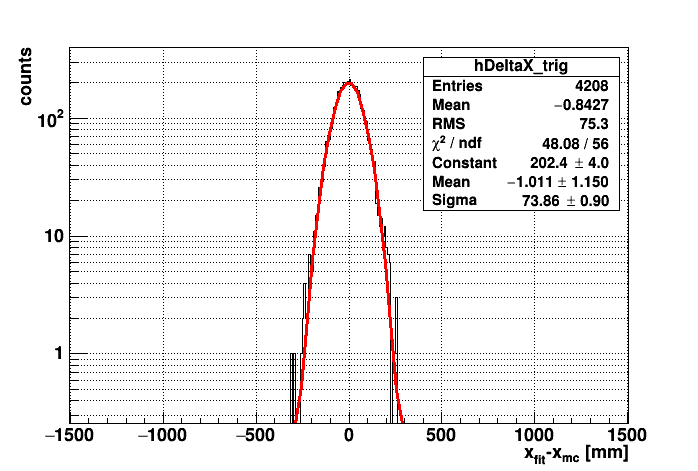
\includegraphics[width=5cm]{partial_top_x.png}
		\end{minipage}
	}   
	\subfloat[water region]{ 
		\begin{minipage}[t]{0.32\textwidth}
			\centering
			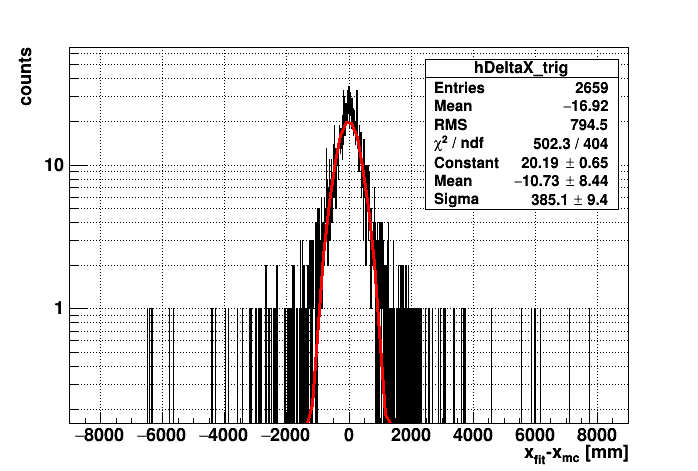
\includegraphics[width=5cm]{partial_bot_x.png}
		\end{minipage}
	}
	\subfloat[whole region]{ 
		\begin{minipage}[t]{0.32\textwidth}
			\centering
			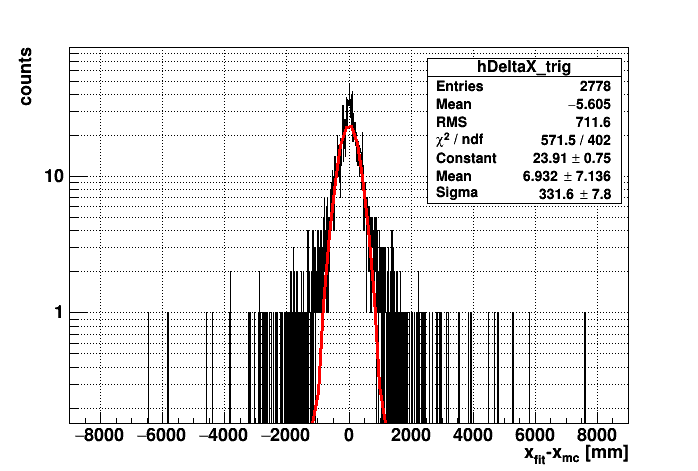
\includegraphics[width=5cm]{partial_full_x.png}
		\end{minipage}
	}
	\caption{Fit position bias projected on x axis ($x_{fit}-x_{MC}$). (a) events simulated in scintillator region only; (b) events simulated in water region only; (c) events simulated in total region.}
	\label{partial_fit_x}
	\subfloat[scintillator region]{ 
		\begin{minipage}[t]{0.32\textwidth}
			\centering
			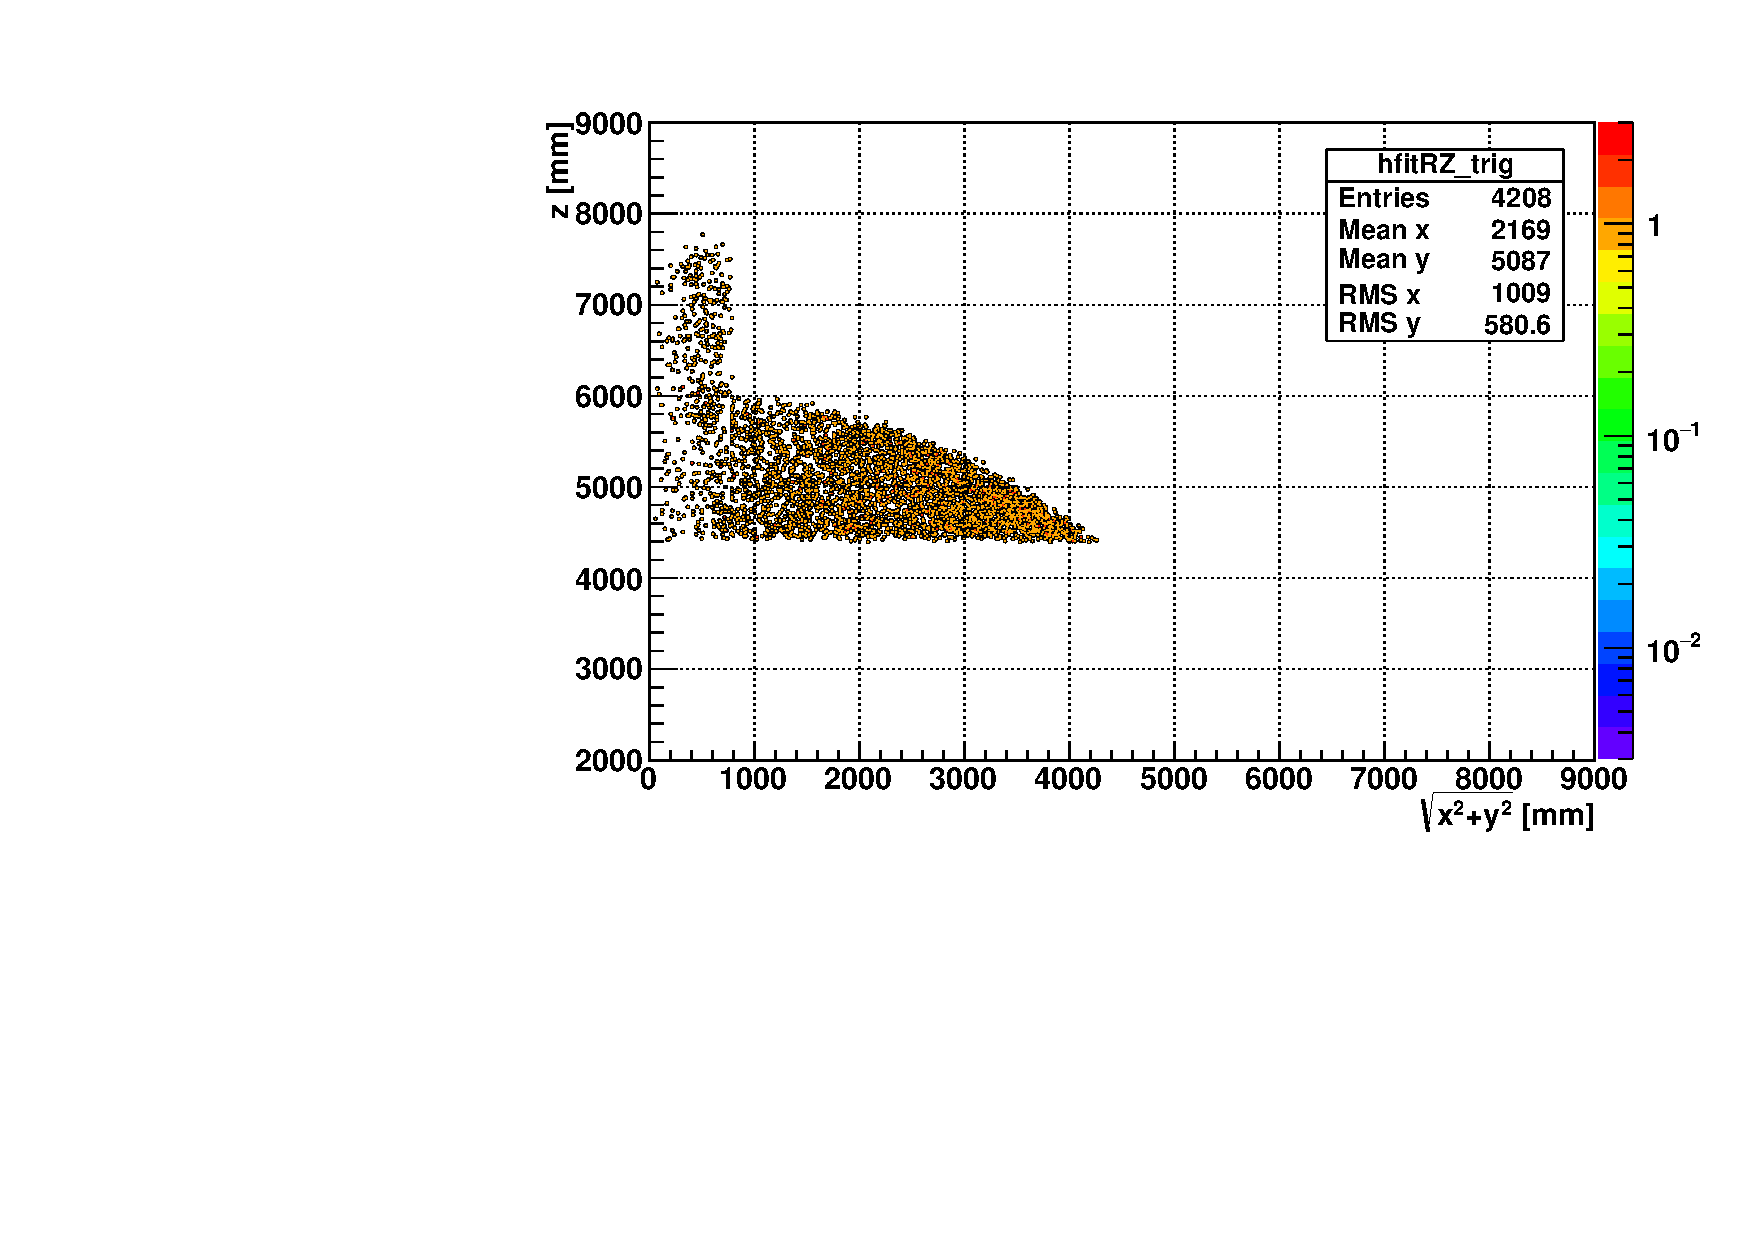
\includegraphics[width=5cm]{partial_top_r.pdf}
		\end{minipage}
	}
	\subfloat[water region]{ 
		\begin{minipage}[t]{0.32\textwidth}
			\centering
			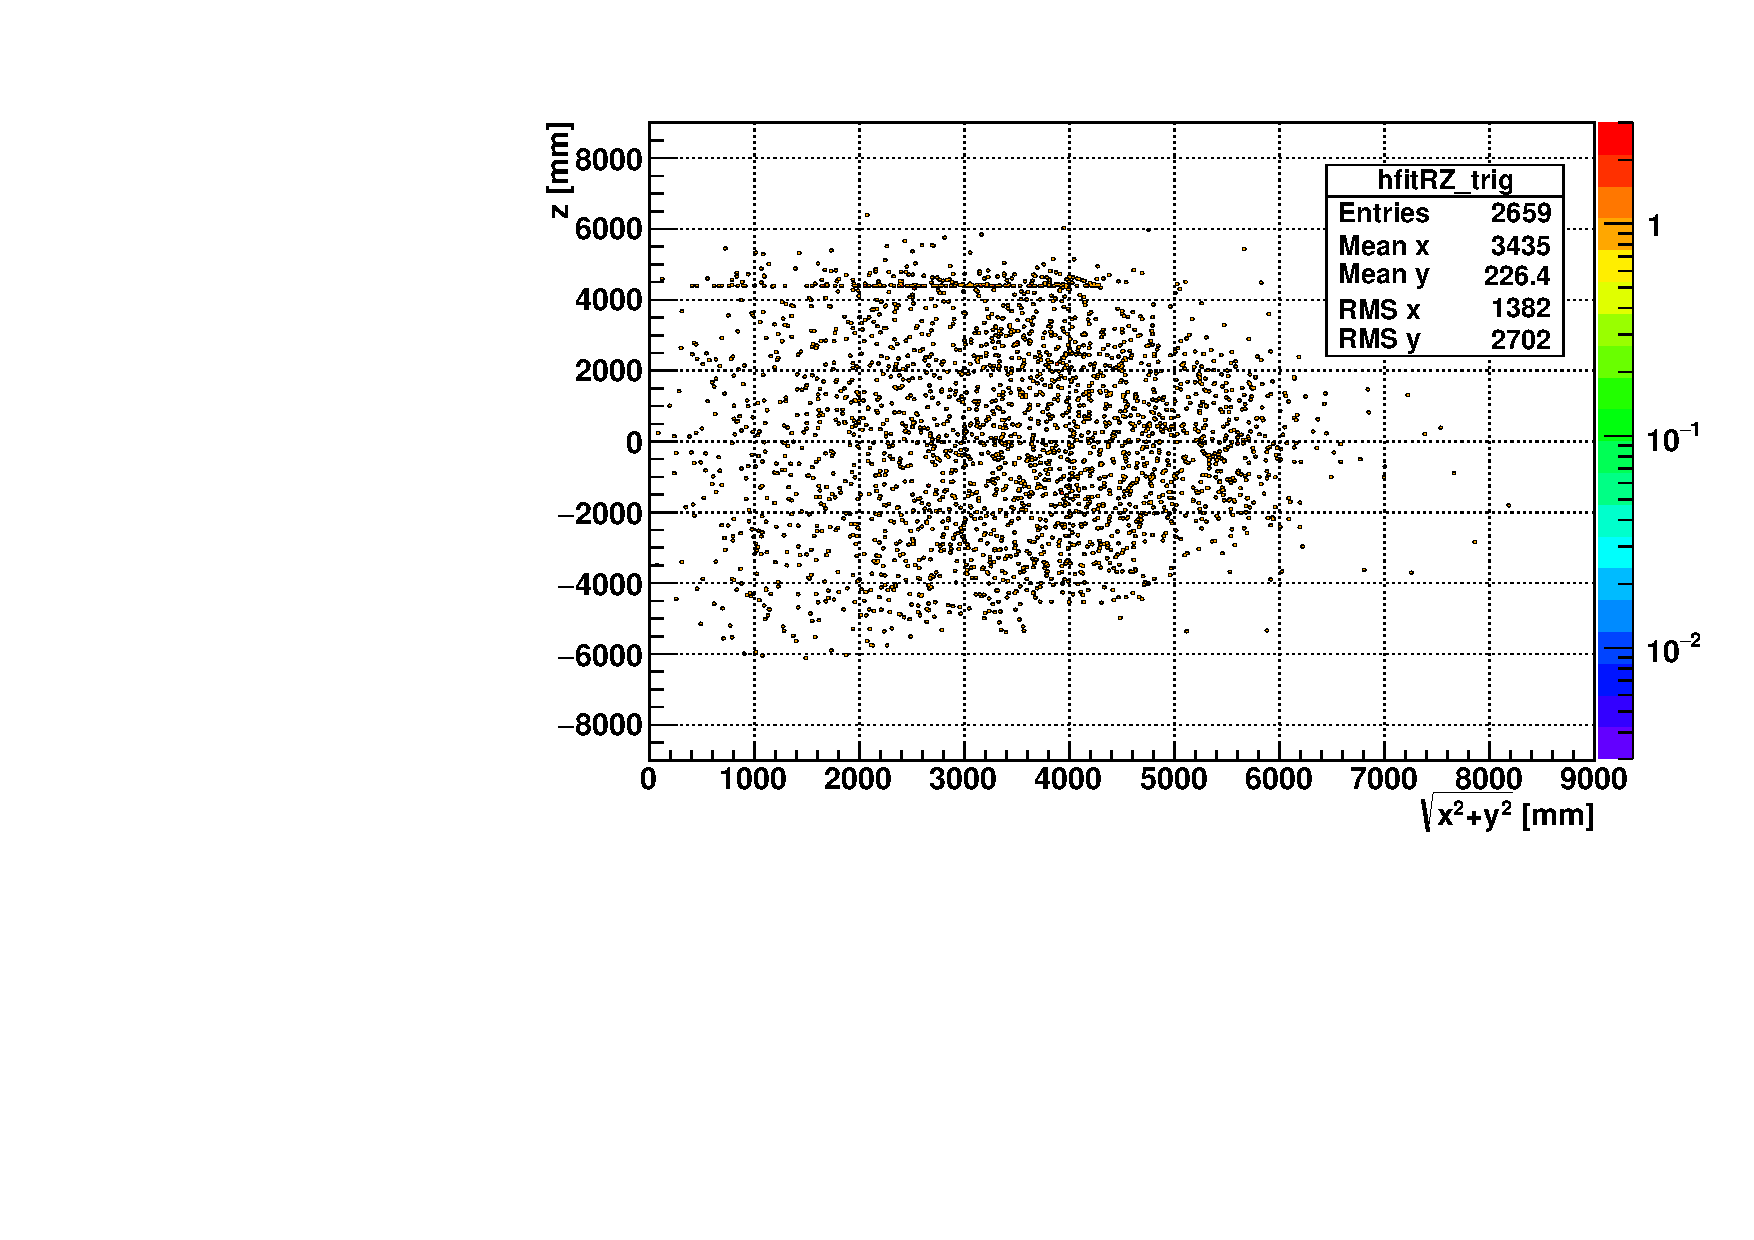
\includegraphics[width=5cm]{partial_bot_r.pdf}
		\end{minipage}
	}
	\subfloat[whole region]{ 
		\begin{minipage}[t]{0.32\textwidth}
			\centering
			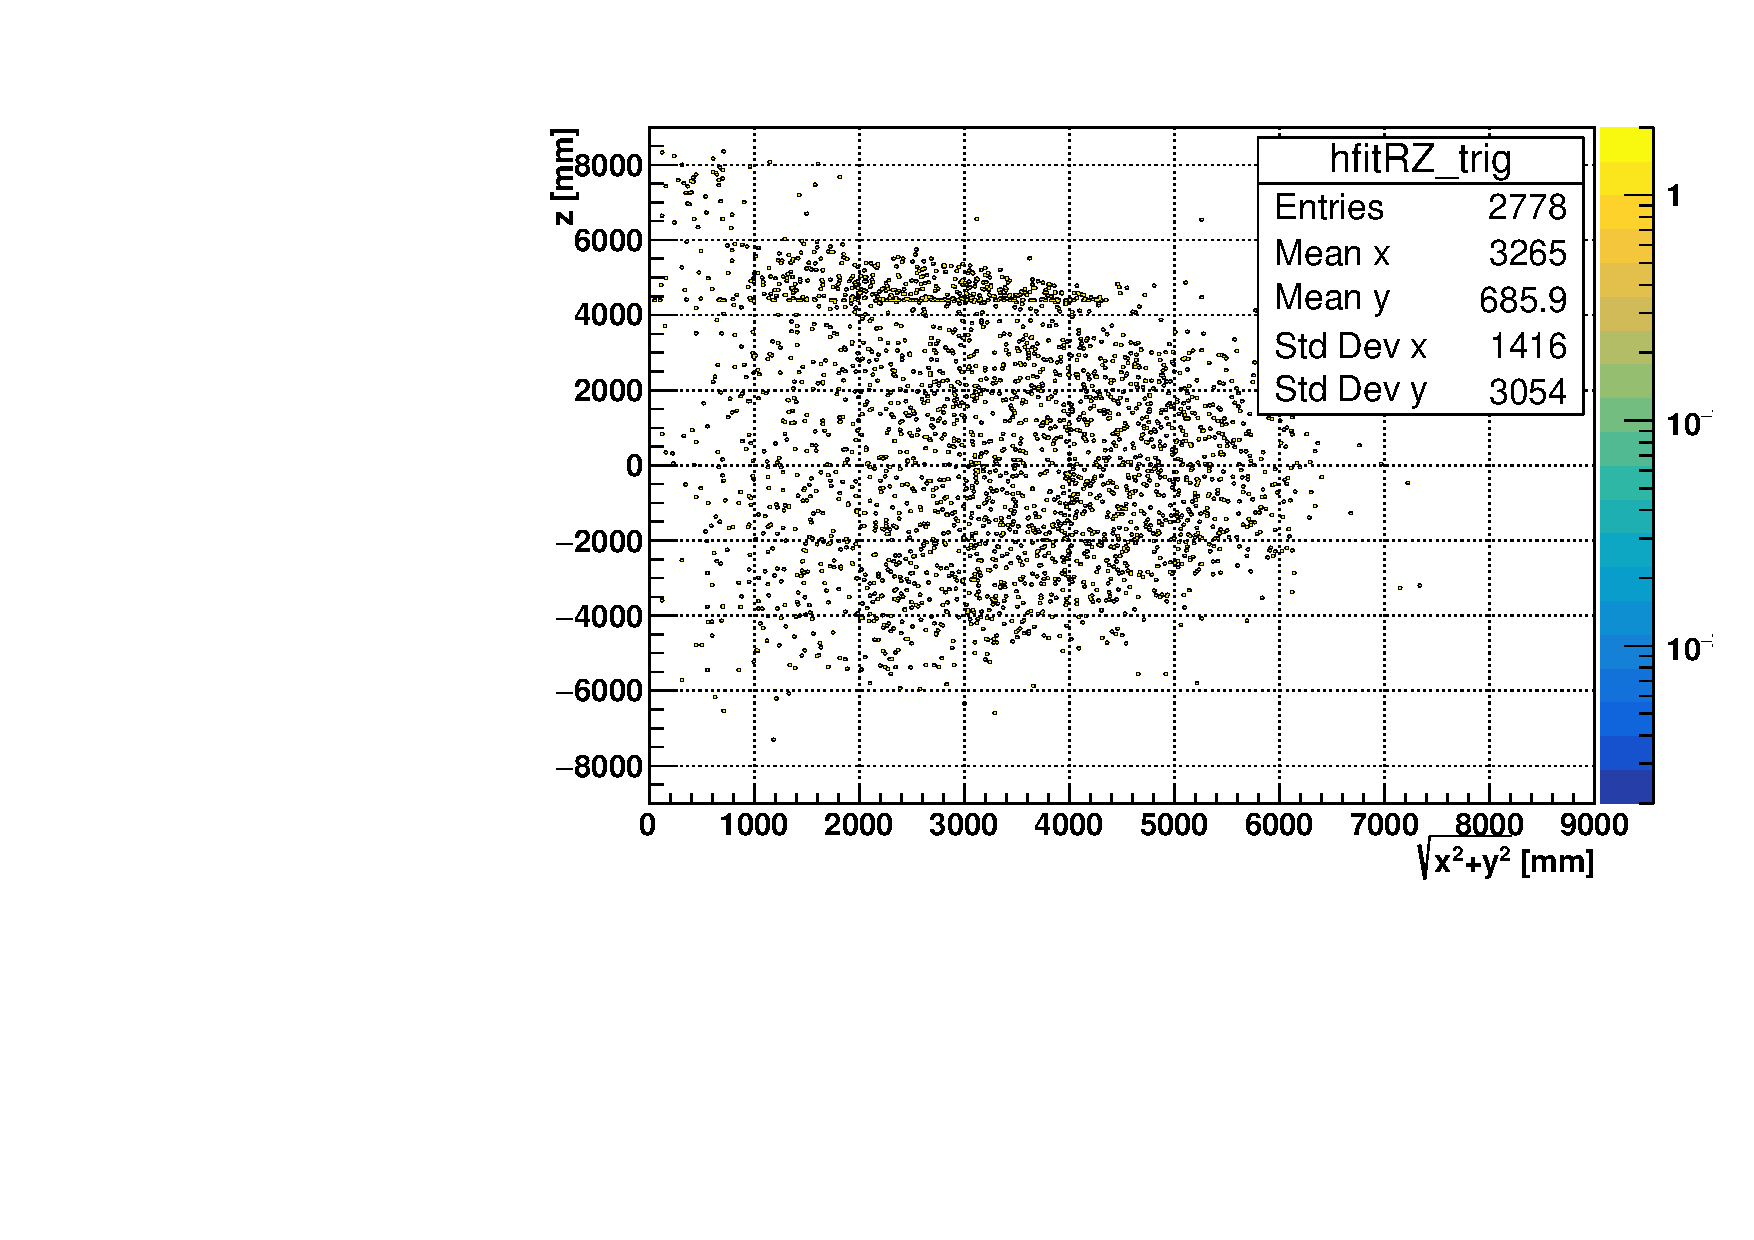
\includegraphics[width=5cm]{partial_full_r.pdf}
		\end{minipage}
	}
	\caption{Fit results of $\rho_{fit}=\sqrt{x_{fit}^2+y_{fit}^2}$ vs. $z_{fit}$.}
	\label{partial_fit_rz}
\end{figure}

The performance of the fitter is studied with MC simulations. In a partial fill geometry with water level at 4.4 m, 2.5 MeV electrons are simulated inside AV in (a) scintillator region only; (b) water region only; (c) whole AV region.

Fig.~\ref{partial_fit_x} and Fig.~\ref{partial_fit_rz} show the MP Partial fitter reconstructed results for these simulations. Fig.~\ref{partial_fit_x} shows the biases between the fit positions and MC positions, projected on the x axis. The distributions of position biases are fitted with Gaussian functions. The values of Gaussian mean and sigma quantify the fit biases and resolutions. The events in scintillator region have  smaller fit biases and better resolutions. Fig.~\ref{partial_fit_rz} shows the fitted $\sqrt{x^2+y^2}$ vs. fitted z positions. It shows that the fitter gives reasonable results of three different MC simulations. 


\section{Plan for Thesis Research}
October to November, 2018: In this short term, my work will focus on the reconstruction algorithm related to the partial fill and scintillator phases. 

November, 2018 to Spring, 2019: I will analyze the partial fill data and the scintillator phase data by utilizing the reconstruction algorithms. The analyses will focus on an understanding of the scintillator backgrounds and searching for solar neutrino signals.

The thesis writing is expected to be finished in summer, 2019.

\vspace{30mm}
\bibliographystyle{elsarticle-num}

\begin{thebibliography}{00}
\bibitem{cowanexpintro} Anderson, E.C. The Reines-Cowan Experiments. 

\url{http://permalink.lanl.gov/object/tr?what=info:lanl-repo/lareport/LA-UR-97-2534-02}
\bibitem{bethe1} H. Bethe and R. Peierls. The `neutrino'. Nature, 133:5321934.
\bibitem{bethe2} Bethe, Hans Albrecht. ``Energy production in stars." Physical Review 55.5 (1939): 434.
\bibitem{bahcall1} Bahcall, John N. ``Solar neutrinos. i. theoretical." Physical Review Letters 12.11 (1964): 300.
\bibitem{raymond} Davis Jr, Raymond. ``Solar neutrinos. ii. experimental." Physical Review Letters 12.11 (1964): 303.
\bibitem{GALLEX} Anselmann, P., et al. ``GALLEX solar neutrino observations. The results from GALLEX I and early results from GALLEX II." Physics Letters B 314.3-4 (1993): 445-458.
\bibitem{SAGE} Abdurashitov, J. N., et al. ``Results from SAGE (The Russian-American gallium solar neutrino experiment)." Physics Letters B 328.1-2 (1994): 234-248.
\bibitem{bahcall2} Bahcall, John N. ``Gallium solar neutrino experiments: Absorption cross sections, neutrino spectra, and predicted event rates." Physical Review C 56.6 (1997): 3391.

\bibitem{imb} Becker-Szendy, R., Bratton, C.B., Casper, D., Dye, S.T., Gajewski, W., Goldhaber, M. et al. (1992) Electron- and muon-neutrino content of the atmospheric flux. Phys. Rev. D 46, 3720-3724.

\bibitem{soudan2} Allison, W.W.M., Alner, G.J., Ayres, D.S., Barrett, W.L., Bode, C., Border, P.M. et al. (Soudan-2 collaboration) (1997) Measurement of the atmospheric neutrino flavour composition in Soudan 2. Phys. Lett. B 391, 491-500.

\bibitem{atmNuReview} Takaaki Kajita, ``Atmospheric Neutrinos," Advances in High Energy Physics, vol. 2012, Article ID 504715, 24 pages, 2012. doi:10.1155/2012/504715

\bibitem{kamioII} Hirata, Kohji S., et al. ``Observation of $^8$B solar neutrinos in the Kamiokande-II detector." Physical Review Letters 63.1 (1989): 16.

\bibitem{herbertChen} Chen, Herbert H. ``Direct approach to resolve the solar-neutrino problem." Physical Review Letters 55.14 (1985): 1534.

\bibitem{SNO} Ahmad, Q. Retal, et al. ``Direct evidence for neutrino flavor transformation from neutral-current interactions in the Sudbury Neutrino Observatory." Physical review letters 89.1 (2002): 011301.

\bibitem{SNOresult} Aharmim, B., et al. ``Combined analysis of all three phases of solar neutrino data from the Sudbury Neutrino Observatory." Physical Review C 88.2 (2013): 025501.

\bibitem{superK} Fukuda, Y., et al. ``Evidence for oscillation of atmospheric neutrinos." Physical Review Letters 81.8 (1998): 1562.

\bibitem{nobeldoc} ``The Nobel Prize in Physics 2015". Nobelprize.org. Nobel Media AB 2014. Web. 1 Oct 2017. \url{http://www.nobelprize.org/nobel_prizes/physics/laureates/2015/}

\bibitem{cahn} Cahn, Robert N., and Gerson Goldhaber. The experimental foundations of particle physics. Cambridge University Press, 2009.

\bibitem{smirnov} Smirnov, A. Yu. ``Solar neutrinos: Oscillations or No-oscillations?." arXiv preprint arXiv:1609.02386 (2016).

\bibitem{xing} Xing, Zhizhong, and Shun Zhou. Neutrinos in particle physics, astronomy and cosmology. Springer Science \& Business Media, 2011.

\bibitem{smirnov_msw} Smirnov, A. Yu. ``The MSW effect and matter effects in neutrino oscillations." Physica Scripta 2005.T121 (2005): 57.

\bibitem{japan_text} Fukugita, Masataka, and Tsutomu Yanagida. Physics of Neutrinos: and Application to Astrophysics. Springer Science \& Business Media, 2013.

\bibitem{nakaya} Nakaya, Tsuyoshi, and Robert K. Plunkett. ``Neutrino oscillations with the MINOS, MINOS+, T2K, and NOvA experiments." New Journal of Physics 18.1 (2016): 015009.

\bibitem{joseTextbook} Valle, José Wagner Furtado, and Jorge Romao. Neutrinos in high energy and astroparticle physics. John Wiley \& Sons, 2015.

\bibitem{pdg2018} M. Tanabashi et al. (Particle Data Group), Phys. Rev. D 98, 030001 (2018).

\bibitem{kamland} Eguchi, K., et al. ``First results from KamLAND: evidence for reactor antineutrino disappearance." Physical Review Letters 90.2 (2003): 021802.

\bibitem{kamland_measure} Abe, S., et al. ``Precision measurement of neutrino oscillation parameters with KamLAND." Physical Review Letters 100.22 (2008): 221803.

\bibitem{dayabayresults} An, Feng Peng, et al. ``Measurement of electron antineutrino oscillation based on 1230 days of operation of the Daya Bay experiment." Physical Review D 95.7 (2017): 072006.

\bibitem{reactorNu} Qian, Xin, and Jen-Chieh Peng. ``Physics with Reactor Neutrinos.'' arXiv preprint arXiv:1801.05386 (2018).

\bibitem{stateofart} A.Ereditato, ``The State of the Art of Neutrino Physics" https://www.worldscientific.com/doi/abs/10.1142/10600

\bibitem{superk_new} Abe, Kazutaka, et al. ``Atmospheric neutrino oscillation analysis with external constraints in Super-Kamiokande I-IV." Physical Review D 97.7 (2018): 072001.

\bibitem{t2k} Abe, K., et al. ``Measurement of neutrino and antineutrino oscillations by the T2K experiment including a new additional sample of $\nu_e$ interactions at the far detector." Physical Review D 96.9 (2017): 092006.

\bibitem{nova} Adamson, P., et al. ``Measurement of the neutrino mixing angle $\theta_{23}$ in NOvA." Physical review letters 118.15 (2017): 151802.


\bibitem{BahcallRoadMap} Bahcall, John N., and Carlos Pena-Garay. ``A road map to solar neutrino fluxes, neutrino oscillation parameters, and tests for new physics.'' Journal of High Energy Physics 2003.11 (2003): 004.

\bibitem{martin} Martin, Brian R. Nuclear and particle physics: an introduction. John Wiley \& Sons, 2006.

\bibitem{majorana} Majorana, Ettore, and Luciano Maiani. ``A symmetric theory of electrons and positrons.'' Ettore Majorana Scientific Papers. Springer, Berlin, Heidelberg, 2006. 201-233.

\bibitem{Qian} Qian, X., \& Vogel, P. (2015). Neutrino mass hierarchy. Progress in Particle and Nuclear Physics, 83, 1-30.

%\bibitem{Brice} Stephen John Brice. Monte Carlo and Analysis Techniques for the Sudbury Neutrino Observatory. PhD thesis, Balliol College, Oxford University, 1996.

%\bibitem{feynmanLatex}J. Ellis, ``TikZ-Feynman: Feynman diagrams with TikZ'', (2016), arXiv:1601.05437 [hep-ph]

\bibitem{kaizuber} Zuber, Kai. ``Neutrinoless double beta decay." arXiv preprint nucl-ex/1201.4665v1 (2012).

\bibitem{gerda} Agostini, M., et al. ``Search of Neutrinoless Double Beta Decay with the GERDA Experiment.'' Nuclear and Particle Physics Proceedings 273 (2016): 1876-1882. 

\bibitem{gerda2} Agostini, M., et al. ``Background-free search for neutrinoless double-$\beta$ decay of 76 Ge with GERDA.'' Nature 544.7648 (2017): 47.

\bibitem{exo} Albert, J. B., et al. ``Search for Majorana neutrinos with the first two years of EXO-200 data.'' Nature 510.7504 (2014): 229.

\bibitem{nEXO} Albert, J. B., et al. ``Sensitivity and Discovery Potential of nEXO to Neutrinoless Double Beta Decay.'' arXiv preprint arXiv:1710.05075 (2017).


\bibitem{kamlandZen} Gando, A., et al. ``Search for Majorana neutrinos near the inverted mass hierarchy region with KamLAND-Zen.'' Physical review letters 117.8 (2016): 082503.

\bibitem{cuore} Alduino, C., et al. ``First Results from CUORE: A Search for Lepton Number Violation via $0\nu\beta\beta$ Decay of $^{130}$Te.'' arXiv preprint arXiv:1710.07988 (2017).

\bibitem{stevenbiller}Biller, Steven, Szymon Manecki, and SNO+ collaboration. ``A New Technique to Load 130Te in Liquid Scintillator for Neutrinoless Double Beta Decay Experiments." Journal of Physics: Conference Series. Vol. 888. No. 1. IOP Publishing, 2017.

\bibitem{whitepaper} Andringa, S., et al. ``Current Status and Future Prospects of the SNO+.'' Advances in High Energy Physics 2016 (2016).

\bibitem{erica} Erica Caden for the SNO+ Collaboration. ``Status of the SNO+ Experiment." arXiv preprint arXiv:1711.11094 (2017).


\bibitem{Dai} Dai, Xiongxin, et al. ``Wavelength shifters for water Cherenkov detectors.'' Nuclear Instruments and Methods in Physics Research Section A: Accelerators, Spectrometers, Detectors and Associated Equipment 589.2 (2008): 290-295.

\bibitem{asdc} Alonso, J. R., et al. ``Advanced scintillator detector concept (ASDC): a concept paper on the physics potential of water-based liquid scintillator." arXiv preprint arXiv:1409.5864 (2014).

\bibitem{boulay} Boulay, Mark Guy. Direct evidence for weak flavour mixing with the Sudbury Neutrino Observatory. 2001.



\end{thebibliography}


\end{document}

%%
%% End of file `elsarticle-template-num.tex'.
